\chapter{Single Mauthner Cell Model - Numerical experiments}\label{ch:expm}
	We will now come to the simulations of the visual looming stimulus experiment.
	For this we first describe the experiments that we want to reproduce, especially the specific 
	conditions and results.
	This is followed by the results of the simulations using the model in the different 
	formulations that we showed in the previous chapter.
	Furthermore, we fit the parameters of the full model to experimental data and finally summarize 
	and discuss our findings.
	\section{Visual looming stimulus experiments}
	One of the earliest visual looming stimulus experiments has been conducted by 
	\cite{Dill1974} where they photographed a black dot on a white background and projected these 
	photographs on a tracing paper that was taped to the wall of the aquarium and thus creating a virtual looming stimulus.
	They also tested a model predator that consisted of a black disk of Plexiglas that was moved by a motor.
	In more recent studies computer-generated stimuli are used and therefore the stimulus size 
	and velocity can be controlled more precisely.\\
	The typical arrangement is a small dish or aquarium in which a single fish can either freely 
	move or it is head-restrained, i.e. it can only move its tail while the head is fixed. 
	In the studies that we will consider here they used larval zebrafish (\cite{Temizer2015}, 
	\cite{Dunn2016}, \cite{Bhattacharyya2017}) and in one case they used goldfish 
	\citep{Preuss2006}.
	The stimulus is then either projected on the floor, ceiling or side wall of the aquarium or a 
	screen is placed close to the aquarium.
	In most studies the stimulus is a black disk or square on a white or blue background.
	Other stimuli that have been tested, such as a circle with a checkerboard pattern did not show significant differences (\cite{Preuss2006}, \cite{Dunn2016}) but there has been no systematic analysis .
	The stimulus sizes, i.e. the diameter of the disk or the side length of the square, range from 0.3 mm to 5 cm and the velocities range from 0.2 cm/s to 60 cm/s.
    Another parameter that is often reported is the ratio of stimulus size and velocity, L/V, which indicates the time needed to cover a distance of a length equal to the stimulus size.
	The subtended visual angles on the retina of the fish range from 2\textdegree to at least 
	100\textdegree.
    In Figure \ref{fig:expm_setup} you can see the experimental setup and the stimuli from the study of \cite{Bhattacharyya2017}.
    \begin{figure}[H]
    	\begin{center}
			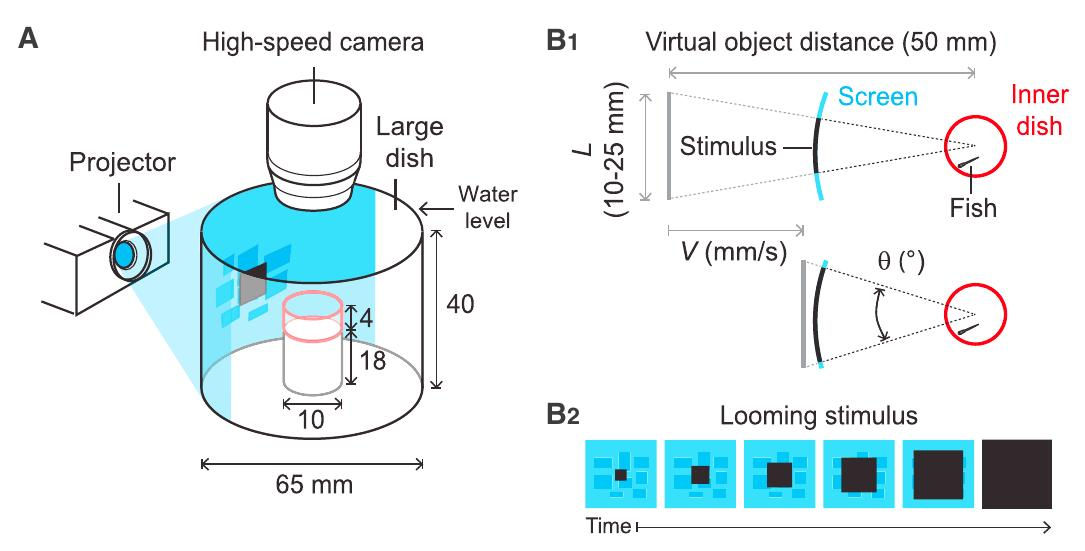
\includegraphics[width=0.8\textwidth]{bhattacharyya_exp_setup.jpeg}
    	\end{center}
    	\caption{\textbf{Experimental setup and stimulus from \cite{Bhattacharyya2017}}. The fish is placed in an inner dish which is located in an larger dish. The stimulus is projected on the wall of the larger dish and the reaction of the fish is recorded from above. Adapted from Figure 1 in \cite{Bhattacharyya2017}.}
    	\label{fig:expm_setup}
    \end{figure}
	For an overview of all reported conditions in the experiments see Table \ref{tab:looming_exp}.\\
	\begin{table} [!th]
		\begin{center}
			\begin{tabular}{l|c|c|c|c}
				%\hline
				\textbf{Study} & \textbf{1} & \textbf{2} & \textbf{3} & \textbf{4}\\
				\hline
				\textbf{Species} & Zebrafish & Zebrafish & Zebrafish & Goldfish\\
				%\hline
				\textbf{Age} & 6-8 dpf & 5-6 dpf & 5 - 7 dpf & -\\
				%\hline
				\textbf{Water temperature [\textdegree C]} & 28  & - & 24  & 18 \\
				%\hline
				\textbf{Screen spanning} & 62 & >100* & >70* & -\\
				\textbf{angle horizontal [\textdegree]} & & & & \\
				%\hline
				\textbf{Screen spanning} & 50 & - & - & -\\
				\textbf{angle vertical [\textdegree]} & & & & \\
				%\hline
				\textbf{Screen distance [cm]} & 1 & - & 3.25 & 16\\
				%\hline
				\textbf{Luminance dark} & 0.07 cd/$m^2$ & 0.7 lux & - & 70-80 lux\\
				%\hline
				\textbf{Luminance grey} & - & 75 lux & - & -\\
				%\hline
				\textbf{Luminance white} & 122.5 cd/$m^2$ & 512 lux & 500 lumen & 300-320 lux\\
				%\hline
				\textbf{L/V values [ms]} & 60-300 \dag & 510 - 2900 \dag & 100 - 
				1200 & 20 - 110*\\
				%\hline
				\textbf{Durations [s]} & 1.65 - 8 & 0.5 - 5* & 1 - 5.5* & 0.25 - 0.8*\\
				%\hline
				\textbf{Acclimation time [min]} & - & - & 15 & -\\
				%\hline
				\textbf{Visual angles [\textdegree]} & 2 - 48 & 25 - 100* & 8 - 70* & 2 - 100*\\
				%\hline
				\textbf{Critical angle [\textdegree]} & 21.7 $\pm$ 2.5 & 72 $\pm$ 1.3 & 35 $\pm$ 15 
				& -\\
				%\hline
				\textbf{Response probabilities} & 20 - 75* & 46 - 60 & 25 - 75* & 70 - 91\\
				%\hline
				\textbf{Head-restrained} & Yes & No & No & No\\
				%\hline
				\textbf{Stimulus shape} & Circle & Circle & Rectangle & Circle\\
				%\hline
				\textbf{Stimulus color} & Black/White, & Black/Chkb. & Black & Black\\
				%\hline
				\textbf{Background color} & White/Black, & Grey & Blue & White\\
				%\hline
				\textbf{Stimulus sizes [cm]} & 0.03 & ? & 1 - 2.5 & 0.5 - 5*\\
				%\hline
				\textbf{Stimulus velocities [cm/s]} & 0.2 - 1 & ? & ? & 20 - 60\\
				%\hline
				\textbf{Initial distances} & ? & ? & 5 & ?\\
				\textbf{(virtual) [cm]} &  &  &  & \\
				%\hline
				\textbf{Projection site} & Side/Front & Bottom & Side/Front & Above\\
				%\hline
			\end{tabular}
		\end{center}
		\caption{The corresponding references of the studies are 1: \cite{Temizer2015}, 
		2: \cite{Dunn2016}, 3: \cite{Bhattacharyya2017} and 4: \cite{Preuss2006}.
		Note that the studies might have conducted other looming stimulus experiments with 
		simultaneous neural recordings but they are not included here because this project is 
		restricted to the behavioral aspects.
		For values denoted with a "\dag" we used the diameter 
		instead of the radius, as it was done in the original studies.
		Values with an "*" are either 
		read of figures or inferred from other, reported values. Chkb. = Checkerboard pattern.}
		\label{tab:looming_exp}
	\end{table}
	%TODO: make appropriate groups for table and/or remove some of them and put the full table into appendix
	For the results of the experiment the time from onset of the stimulus (latency), the distance and the 
	visual angle are measured at the time when the fish responds, i.e. starts to move away.
	The visual angle at response time (response angle) has been found to have the same mean value 
	at different stimulus sizes and velocities in all studies that were done with zebrafish, 
	although there are substantial differences in the mean value as well as in the variance.
	This could be explained by the differences in various experimental conditions such as the water 
	temperature, head restraining or the acclimation time (see Table \ref{tab:looming_exp}).
	While the study with goldfish \citep{Preuss2006} does not report to find a so-called critical visual angle, the observed response angles (14\textdegree{} to 29\textdegree) are in a range 
  	that is comparable to e.g. the one found by \cite{Bhattacharyya2017} (35\textdegree{} $\pm$ 
	15\textdegree).
    The distribution of response angles in dependence of the L/V values of all studies considered here is shown in Figure \ref{fig:expm_theta_lv}.\\
    \begin{figure}[!h]
    	\begin{center}
			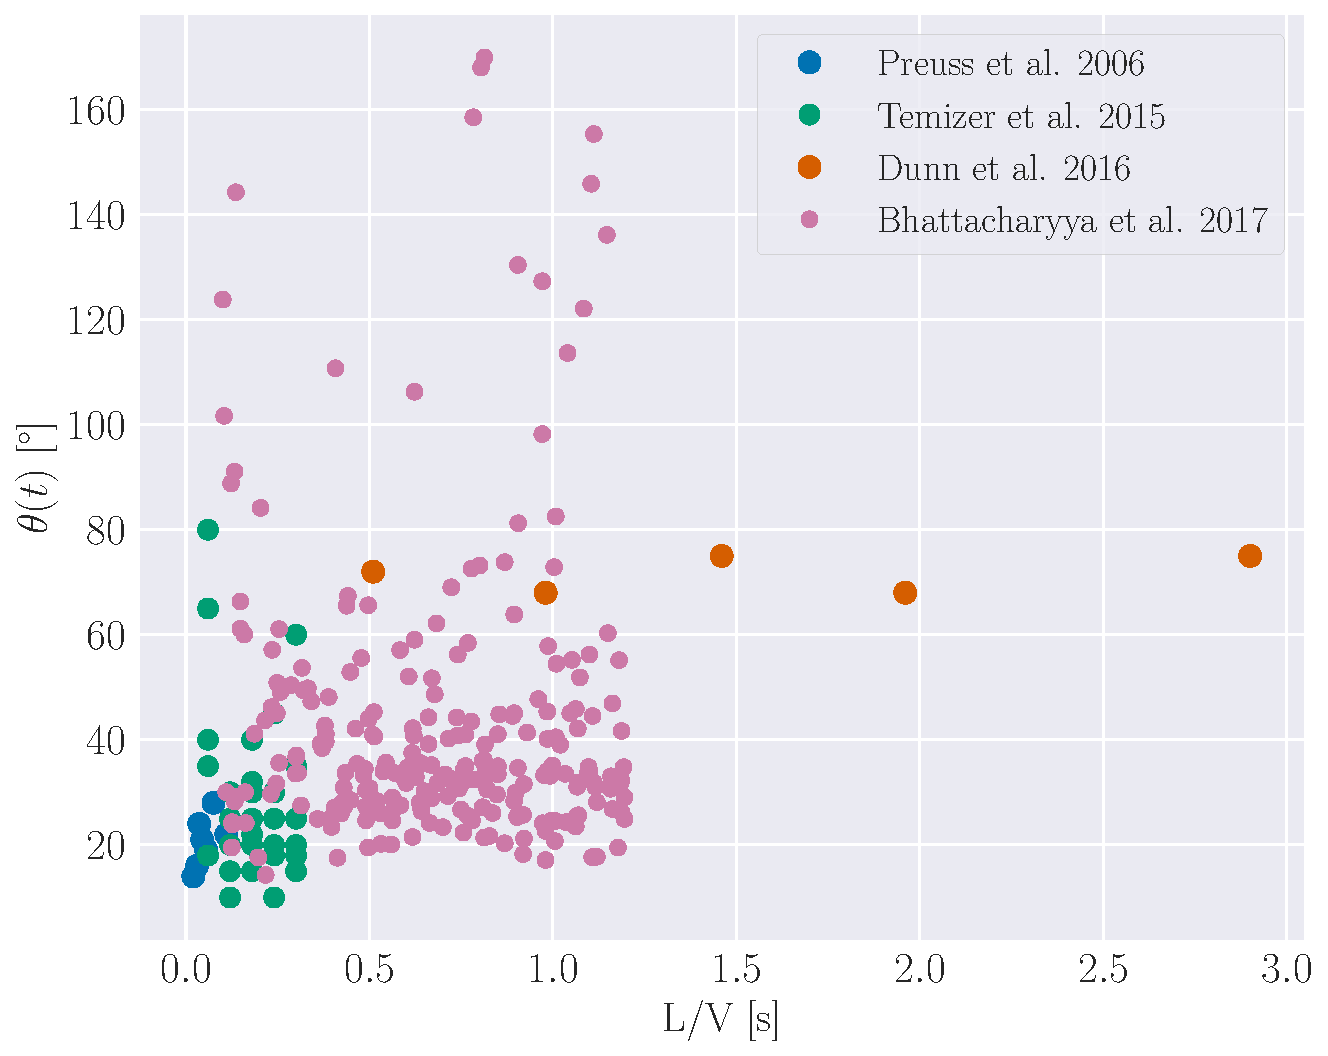
\includegraphics[width=0.8\textwidth]{figure_expm_theta_vs_lv.pdf}
    	\end{center}
    	\caption{Experimental response angles against L/V values.}
    	\label{fig:expm_theta_lv}
    \end{figure}
	For the simulations of the experiment we closely followed the procedure reported by 
	\cite{Bhattacharyya2017}.
	At the beginning of a trial a stimulus size is drawn from a uniform distribution between 10 mm and 25 mm.
	Next, an L/V value is uniformly drawn between 0.1 s and 1.2 s and the resulting velocity for the 
	trial stimulus size is calculated.
	With the trial stimulus size $L_{trial}$ and the trial velocity $v_{trial}$ the visual angle 
	over time $\theta(t)$ is calculated by:
	\begin{equation}
	\theta (t) = 2\cdot \arctan(\frac{L_{trial}/2}{D_{init} - v_{trial}\cdot t}),
	\label{eq:theta}
	\end{equation}
	where $D_{init}$ is the virtual initial distance which is set to 50mm if not stated otherwise.
    The range of possible time courses of the visual angle is shown in Figure \ref{fig:theta_lv} A.
    Note that because the initial distance is fixed and we sample from different stimulus sizes we get different initial angles for the same L/V values.
    This leads to different time courses for the same L/V value depending on the stimulus size but starting from the same angle their time courses are identical (Figure \ref{fig:theta_lv} B).
    If we now assume a critical angle $\theta_{crt}$ at which the fish escapes, we can describe how the response time, response distance and time-to-collision (TTC) at response depend on the L/V value.
    The response time linearly depends on the L/V while the slope of the relationship is determined by stimulus size $L$, initial distance $D_{init}$ and critical angle $\theta_{crt}$:
	\begin{equation}
	t_{resp} = \dfrac{L}{v} \left(\dfrac{D_{init}}{L} - \dfrac{1}{2\cdot\tan(\theta_{crt} /2)}\right).
	\label{eq:resp_time}
	\end{equation}
    The response distance only depends on the stimulus size $L$:
    \begin{equation}
	D_{resp} = \dfrac{L}{2\cdot \tan(\theta_{crt} /2)}.
	\label{eq:resp_dist}
	\end{equation}
    The TTC linearly depends on $L/V$ and the slope is determined only by the critical angle $\theta_{crt}$:
	\begin{equation}
	TTC_{resp} = - \dfrac{L}{2\cdot v\cdot \tan(\theta_{crt} /2)}.
	\label{eq:resp_ttc}
	\end{equation}
    For an example with $\theta_{crt}=35$ and $D_{init}=50$ these idealized response properties are illustrated in Figure \ref{fig:ideal_resp_props}, where we chose the same axes as in Figure 1 of \cite{Bhattacharyya2017} for easy comparison.\\
	In our simulations the visual angle is next transformed by a linear function and the result is the input $I(t)$ for our neuronal model, described in the previous chapter:
	\begin{equation}
	I(t) = f(\theta (t)) = c_{scale}(m \cdot \theta(t) + b).
	\label{eq:input}
	\end{equation}
	In order to calculate the response properties we take the time of the first spike $t_{spk}$ of the model M-cell after stimulus onset as the response time of the fish.
	We ignore further processing time after the spike because it is in the order of milliseconds \citep{Preuss2003} and thus irrelevant with respect to the overall response time which is in the order of at least hundreds of milliseconds for visual stimuli \citep{Preuss2006}.
	Thus the response angle of the simulated trial will be $\theta (t_{spk})$.
	%TODO: mention initial period with constant size
	
    \begin{figure}[H]
    	\begin{center}
			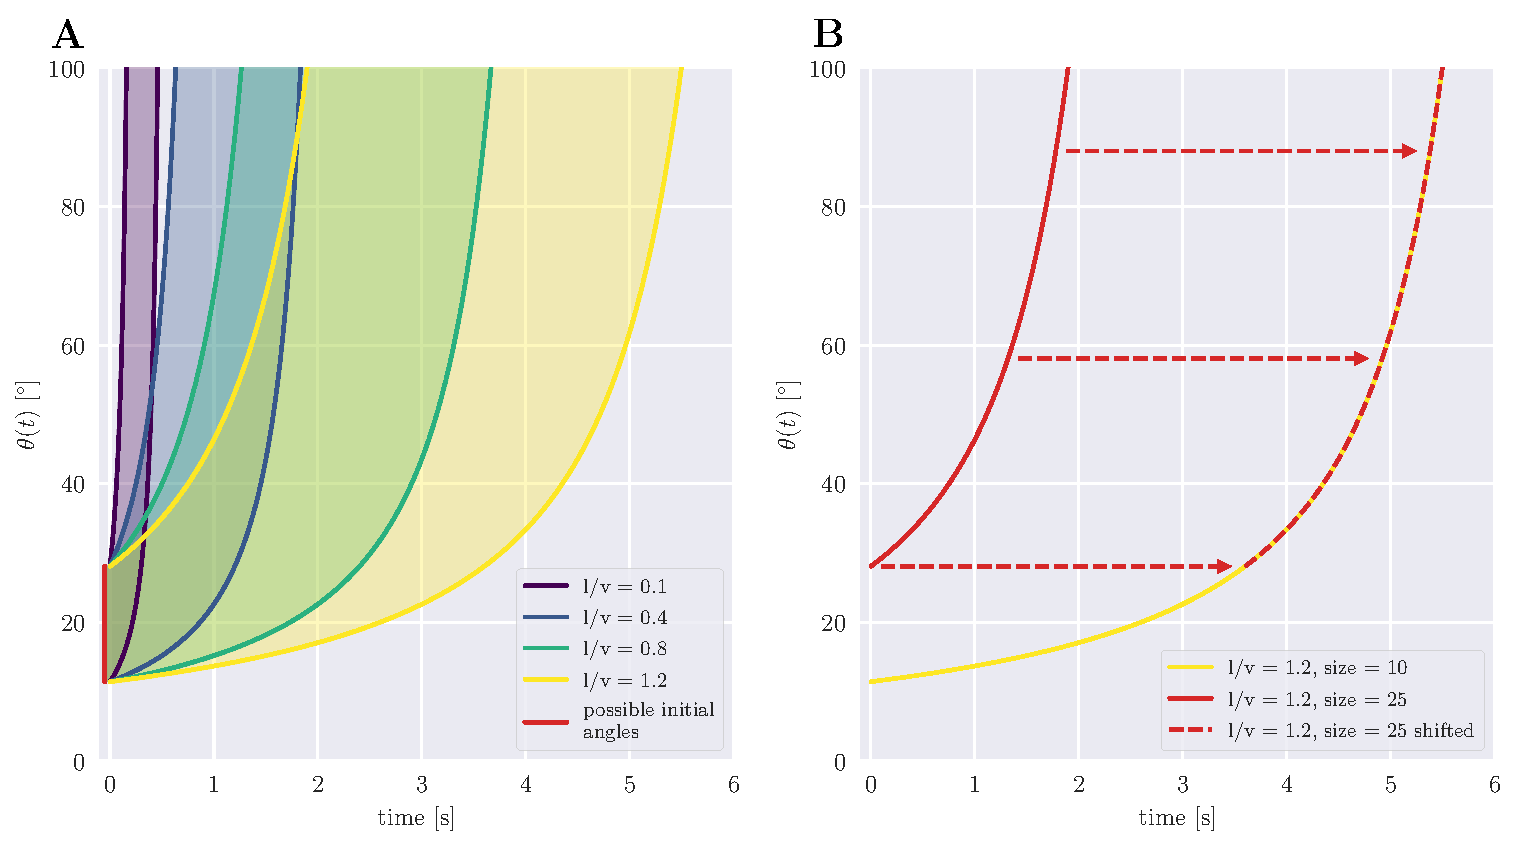
\includegraphics[width=\textwidth]{figure_theta_lv_test.pdf}
    	\end{center}
    	\caption{Range of time courses of $\theta$ depending on L/V. \textbf{A} For four different L/V values the possible time courses are shown if stimulus size L ranges between 10 mm and 25 mm. \textbf{B} Single time courses for the same L/V value only differ in a horizontal shift that is introduced by the different initial angle.}
    	\label{fig:theta_lv}
    \end{figure}
    
    \begin{figure}[H]
    	\begin{center}
			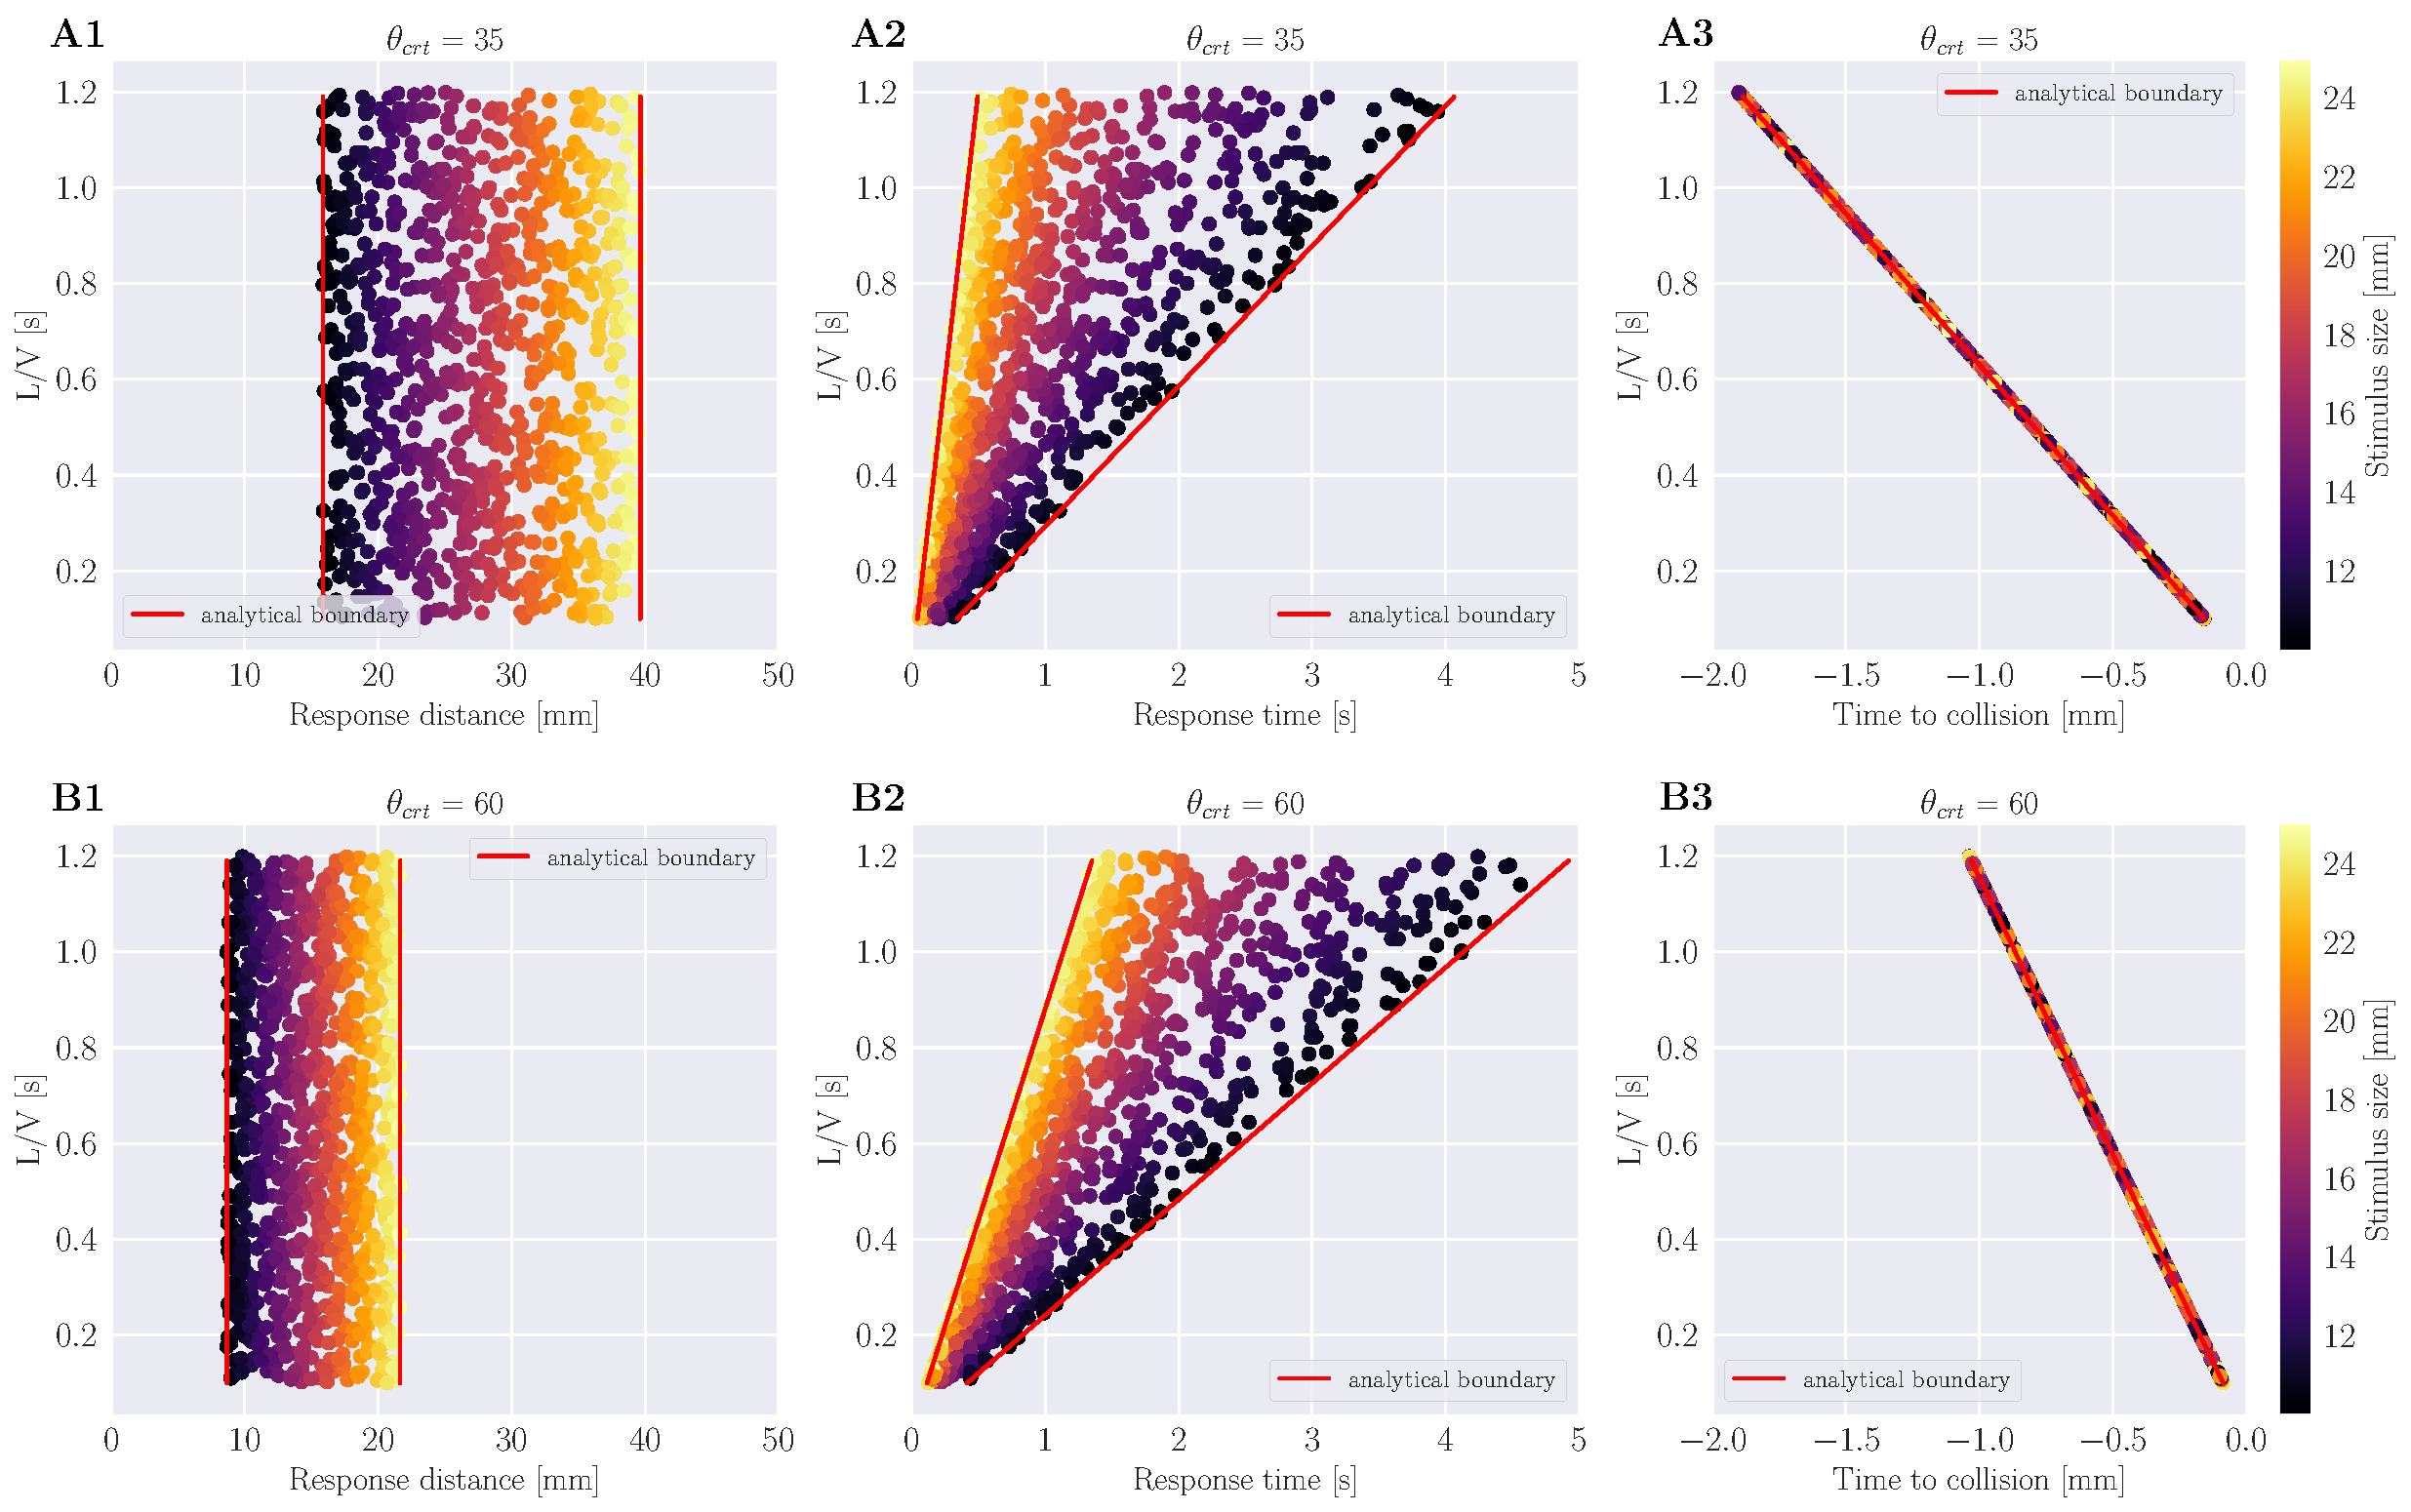
\includegraphics[width=\textwidth]{figure_ideal_resp_v2.pdf}
    	\end{center}
    	\caption{Response properties for a critical angle $\theta_{crt}=35$ and initial distance $D_{init}=50$ mm.  For all plots L was sampled between 10 mm and 25 mm and L/V was sampled between 0.1 s and 1.2 s. Red lines show minimal and maximal values that were calculated using equations \ref{eq:resp_time}, \ref{eq:resp_dist} and \ref{eq:resp_ttc}. \textbf{A} The response distance only depends on L and thus has the same range for all L/V values. \textbf{B} Response times linearly increase with L/V and the slope increases for smaller L. \textbf{C} Absolute time-to-collision linearly increases with L/V and the slope only depends on $\theta_{crt}$.}
    	\label{fig:ideal_resp_props}
    \end{figure}
		
	\section{Stationary Approximation of Full Model}
    For the stationary approximation of the full model in section \ref{approx full model} we derived an analytical solution for the input at which the M-cell fires if there is no noise in the system (see equation \ref{eq:crit_input}).
    Since we defined the time of the first spike of the M-cell as the time at which the fish responds this approximated model therefore has a deterministic response angle.
    Using our definition of the input in the visual looming stimulus experiment from equation \ref{eq:input} we find the following expression for the response angle:
    \begin{equation}
	I(t) = f(\theta(t)) \overset{!}{=} \frac{V_t - E_{L} + \rho_{0}}{(R_{m} - c_{\rho})}
	\label{eq:crit_theta_start}
	\end{equation}
    \begin{equation}
	\Leftrightarrow \theta \overset{!}{=} \frac{V_t - E_{L} + \rho_{0}}{c_{scale}\cdot m \cdot (R_{m} - c_{\rho})} - \frac{b}{m}
	\label{eq:crit_theta_end}
	\end{equation}
	Because we fix the parameters $E_{L}=-79$ mV, $R_{m}=10$ M$\Omega$ and $V_{t}=-61$ mV, the remaining free parameters for this model are $\rho_{0}$, $c_{\rho}$, $c_{scale}$, $m$ and $b$.
    The response angle linearly increases with $\rho_{0}$ and linearly decreases with $b$.
    The influence of $b$ is scaled by $m$ and for $\rho_{0}$ the increase is scaled by the product of $(R_{m} - c_{\rho})$, $c_{scale}$ and $m$.
    Furthermore, the response angle is reversely proportional to $c_{scale}$ and $m$.
    If $c_{\rho} > R_{m}$ the model predicts a negative response angle because this would mean that the effective input for the M-cell is negative.
    As this is unrealistic we constraint $c_{\rho}$ to be strictly smaller than $R_{m}$.
    For the allowed range the response angle increases with increasing $c_{\rho}$ and the increases become larger as $c_{\rho}$ approaches $R_{m}$.
    For a simplified case where we fix $b=0$ and $c_{scale}=3\cdot10^{-10}$, the effect of the remaining free parameters on the response angle is shown in Figure \ref{fig:effect_stationary_params}.\\
    If we now look at the effects of adding noise to the system, first we have to specify the random distribution for the resting activity of the inhibitory population $\rho_0$.
    Motivated by the rarely occurring but very high response angles in the data of \cite{Bhattacharyya2017} (see Figure \ref{fig:expm_theta_lv}) we chose the log-normal distribution that is parametrized by the mean $\mu_{\rho_{0}}$ and the standard deviation $\sigma_{\rho_{0}}$ of the normal distribution it is derived from:
    \begin{equation}
	 ln(P_{0}) \sim \mathcal{N}(\mu_{\rho_{0}},\,\sigma_{\rho_{0}}^{2}).
	\label{eq:rho_null}
	\end{equation}
    The main difference from a normal distribution is that the log-normal distribution has much higher probabilities for high values, also called a "fat tail" and this will allow the model to account for the rare but high response angles.\\
    For the stationary model, all sources of noise that we consider here: membrane potential, firing threshold, inhibitory population activity and the resting activity of the inhibitory population, all have qualitatively the same linear effect on the response angle that is exemplified by the effect of $\rho_0$ in Figure \ref{fig:effect_stationary_params} C.
    This means that the distribution of response angles will closely follow the noise distribution.
    For the Gaussian noise on the membrane potential the response angles are approximately normally distributed and the mean and variance of the distribution depend on the variance of the added noise.
    The mean response angle decreases with increasing variance and the variance of the distribution increases with increasing variance of the noise (Figure \ref{fig:effect_noise_stationary} A1 and B1).
    Combining two sources of noise increases these effects (Figure \ref{fig:effect_noise_stationary} A2 and B2).\\
    Note, that the decrease of the mean response angle is due to the noise being instantaneous in our case, which effectively models fast threshold fluctuations with extremely short relaxation times.
    If we look at noise on the threshold for an example, this means that at each point in time, there is a high probability that the threshold is much lower than its average value which effectively lowers the threshold on average.
    If, on the other hand, the threshold was described by a stochastic process with a large relaxation time we could say that the threshold would be constant for the time of a single trial and the value would be a sample from the distribution.
    In Figure \ref{fig:static_vs_dynamic_noise} we compare these two extreme cases and see that for the "constant" noise, the mean value of the response angle distribution does not change (Figure \ref{fig:static_vs_dynamic_noise} B).\\
    For the log-normally distributed noise on the resting activity of the inhibitory population the response angles again follow the noise distribution (Figure \ref{fig:effect_rho_null_stationary}).
    At higher variances there are trials in which the inhibition is so strong that the M-cell does not fire at all within the trial time (bars at 180\textdegree{} in Figure \ref{fig:effect_rho_null_stationary}).
    \begin{figure}[H]
    	\begin{center}
			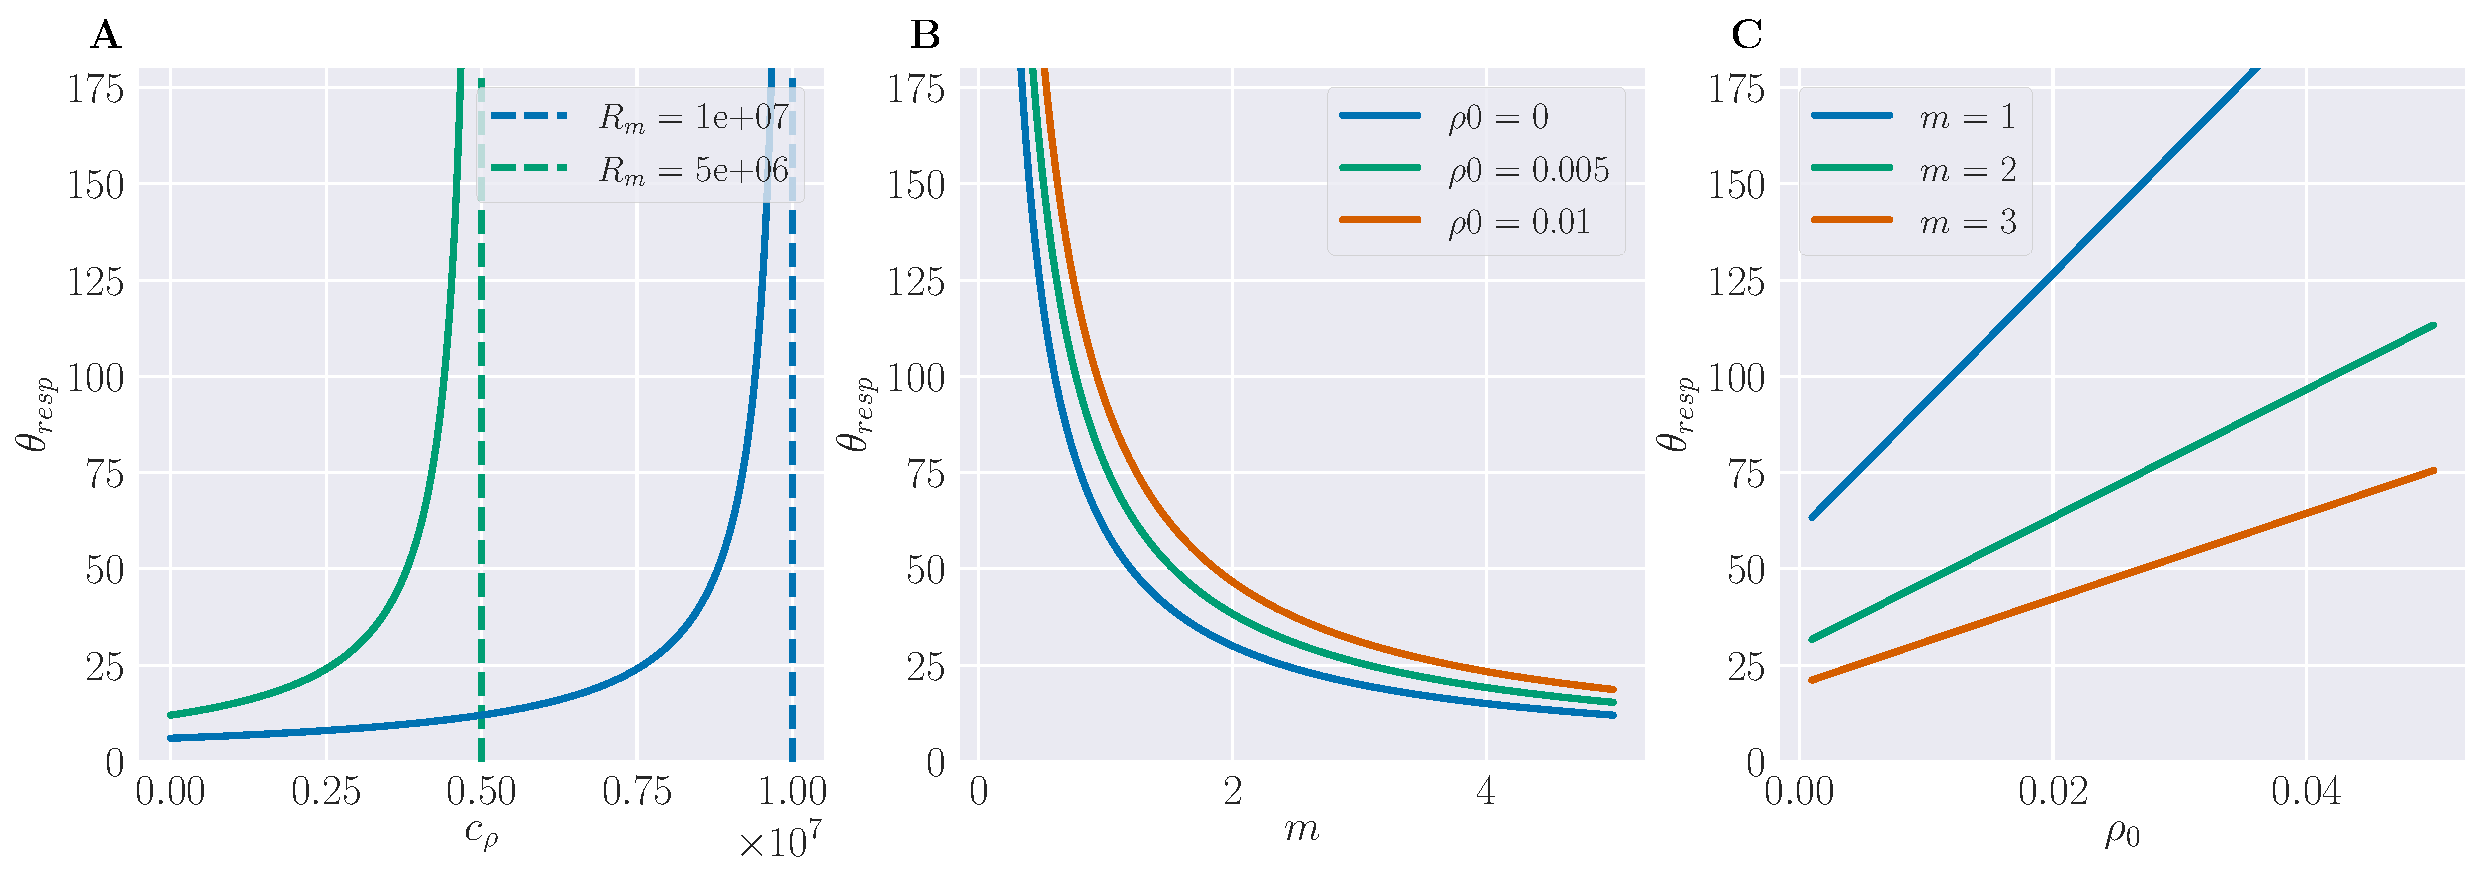
\includegraphics[width=\textwidth]{figure_stationary_params.pdf}
    	\end{center}
    	\caption{\textbf{Effect of parameters on response angle in the noise-free, stationary model.}  For $b=0$ and $c_{scale}=3\cdot10^{-10}$. \textbf{A} Response angle increases exponentially with the scaling of the input for the inhibitory population. For two different values of the membrane resistance $R_{m}$. \textbf{B} Response angle decreases exponentially with the slope of the linear transformation of the visual angle. \textbf{C} Response angle increases linearly with higher resting activity of the inhibitory population.}
    	\label{fig:effect_stationary_params}
    \end{figure}
    
    \begin{figure}[H]
    	\begin{center}
			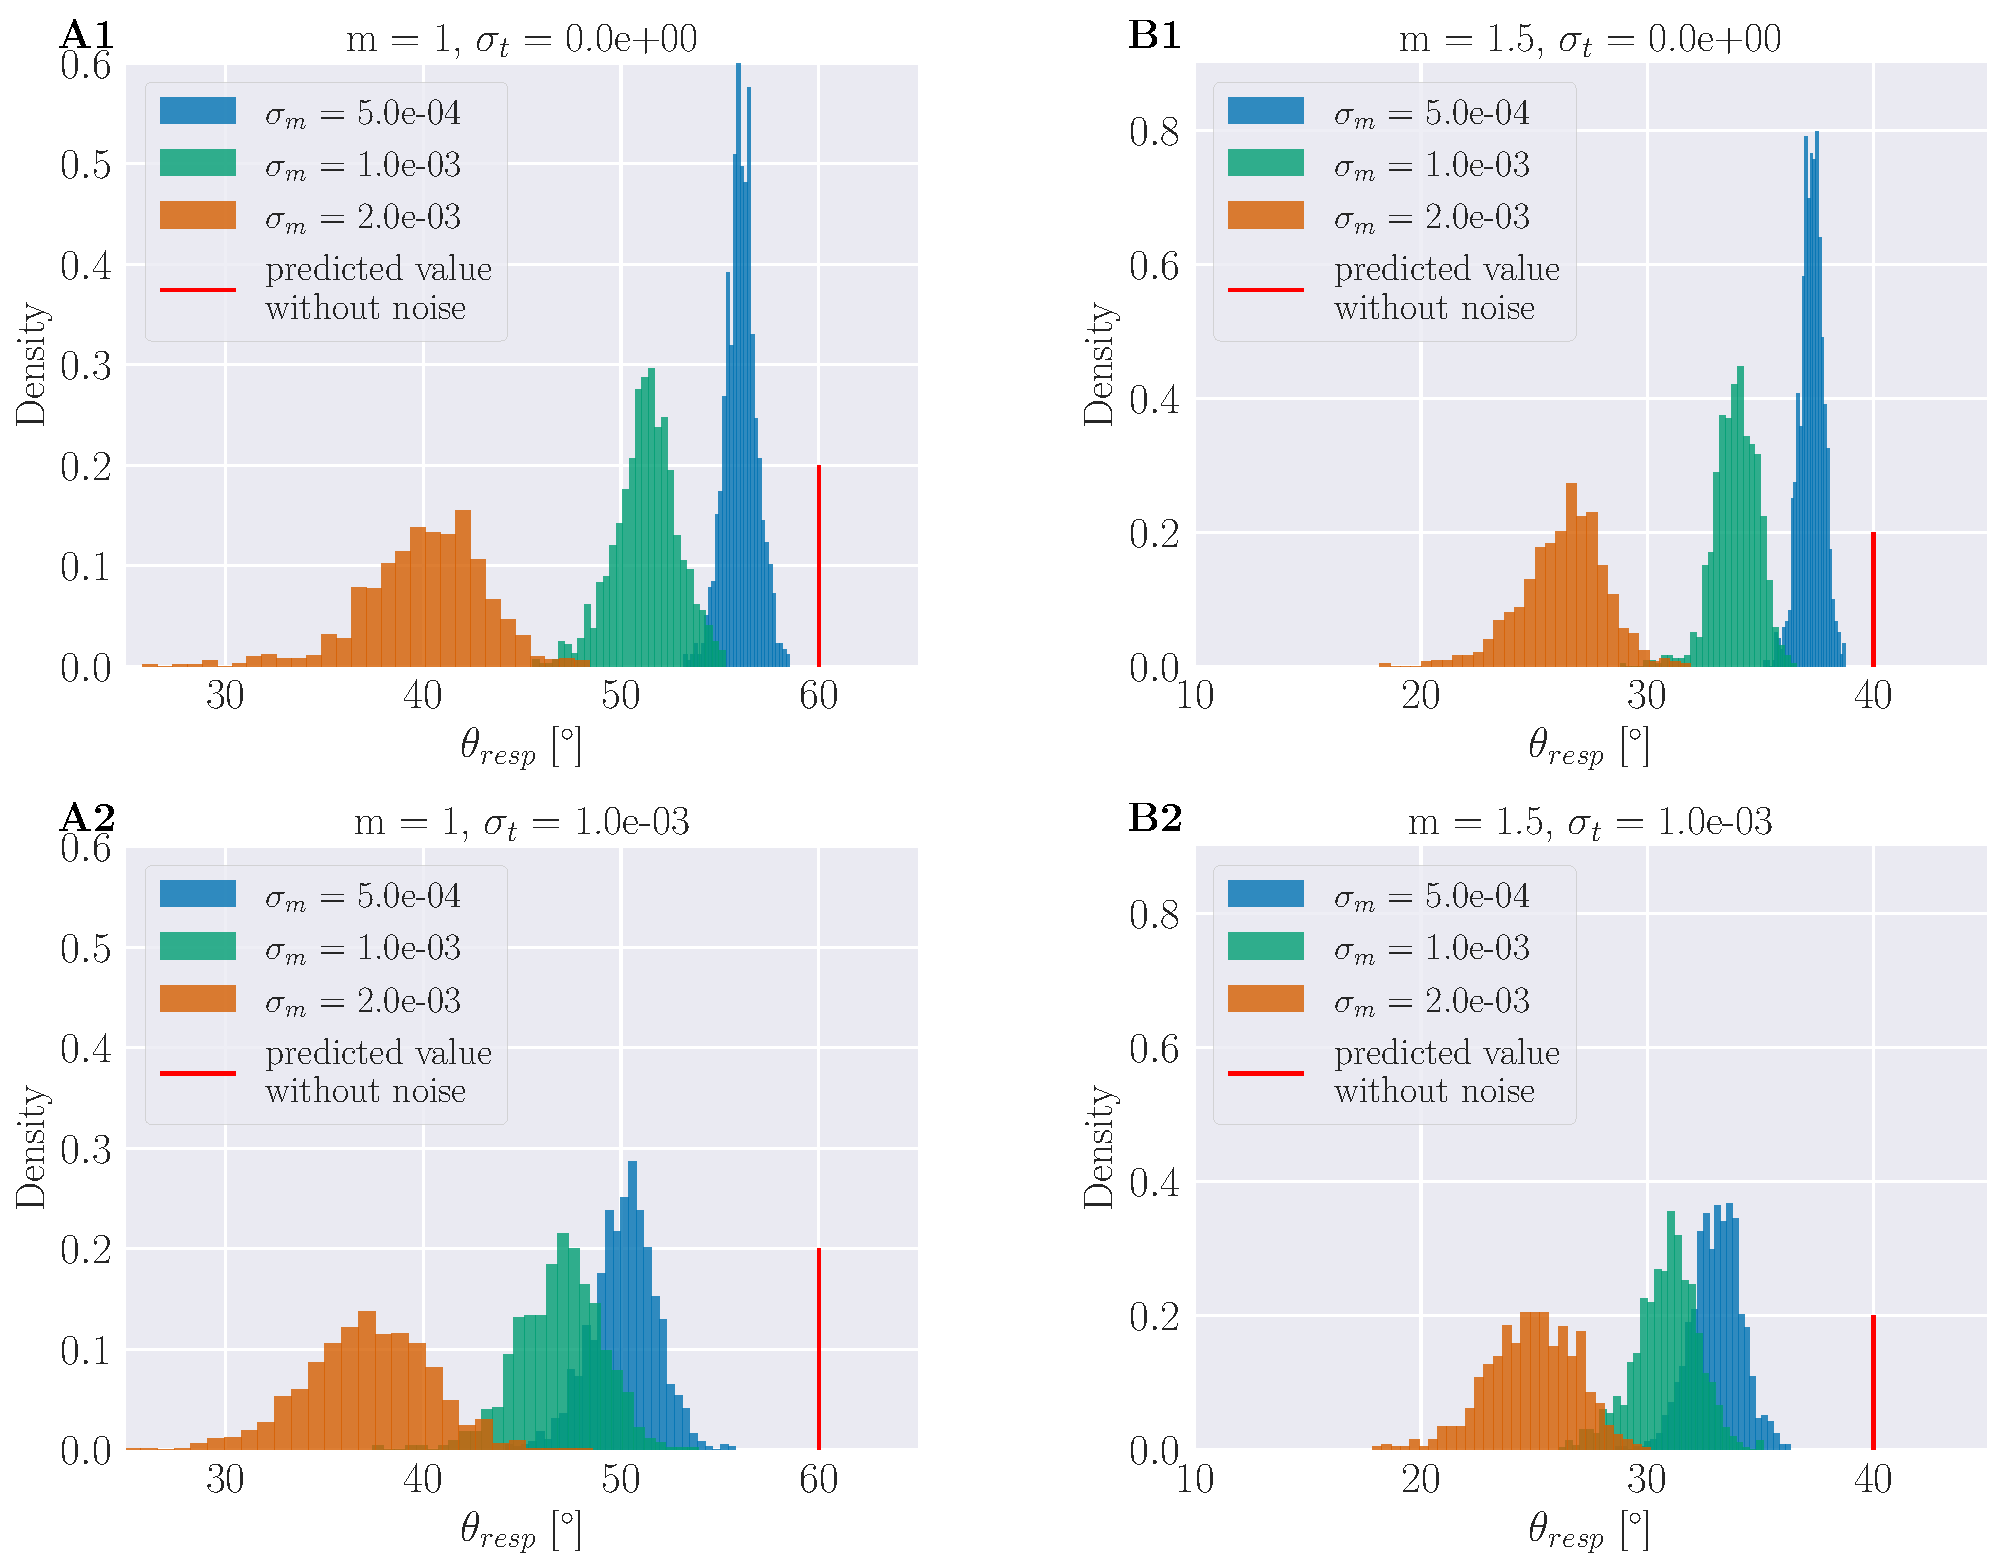
\includegraphics[width=\textwidth]{figure_stationary_noisy_params.pdf}
    	\end{center}
    	\caption{\textbf{Response angle distributions for membrane potential and threshold noise.} For $b=0$, $c_{scale}=3\cdot10^{-10}$, $\rho_{0}=0$, $c_{\rho}=0.9\cdot 10^{7}$. Increasing the variance of the noise decreases the mean response angle and increases the variance of the distribution of response angles. This is independent of the value of the response angle without noise (\textbf{A} vs. \textbf{B}). The effects of two noise sources together add up in a nonlinear way (\textbf{A1} vs. \textbf{A2} and \textbf{B1} vs. \textbf{B2}).}
    	\label{fig:effect_noise_stationary}
    \end{figure}
    
    \begin{figure}[H]
    	\begin{center}
			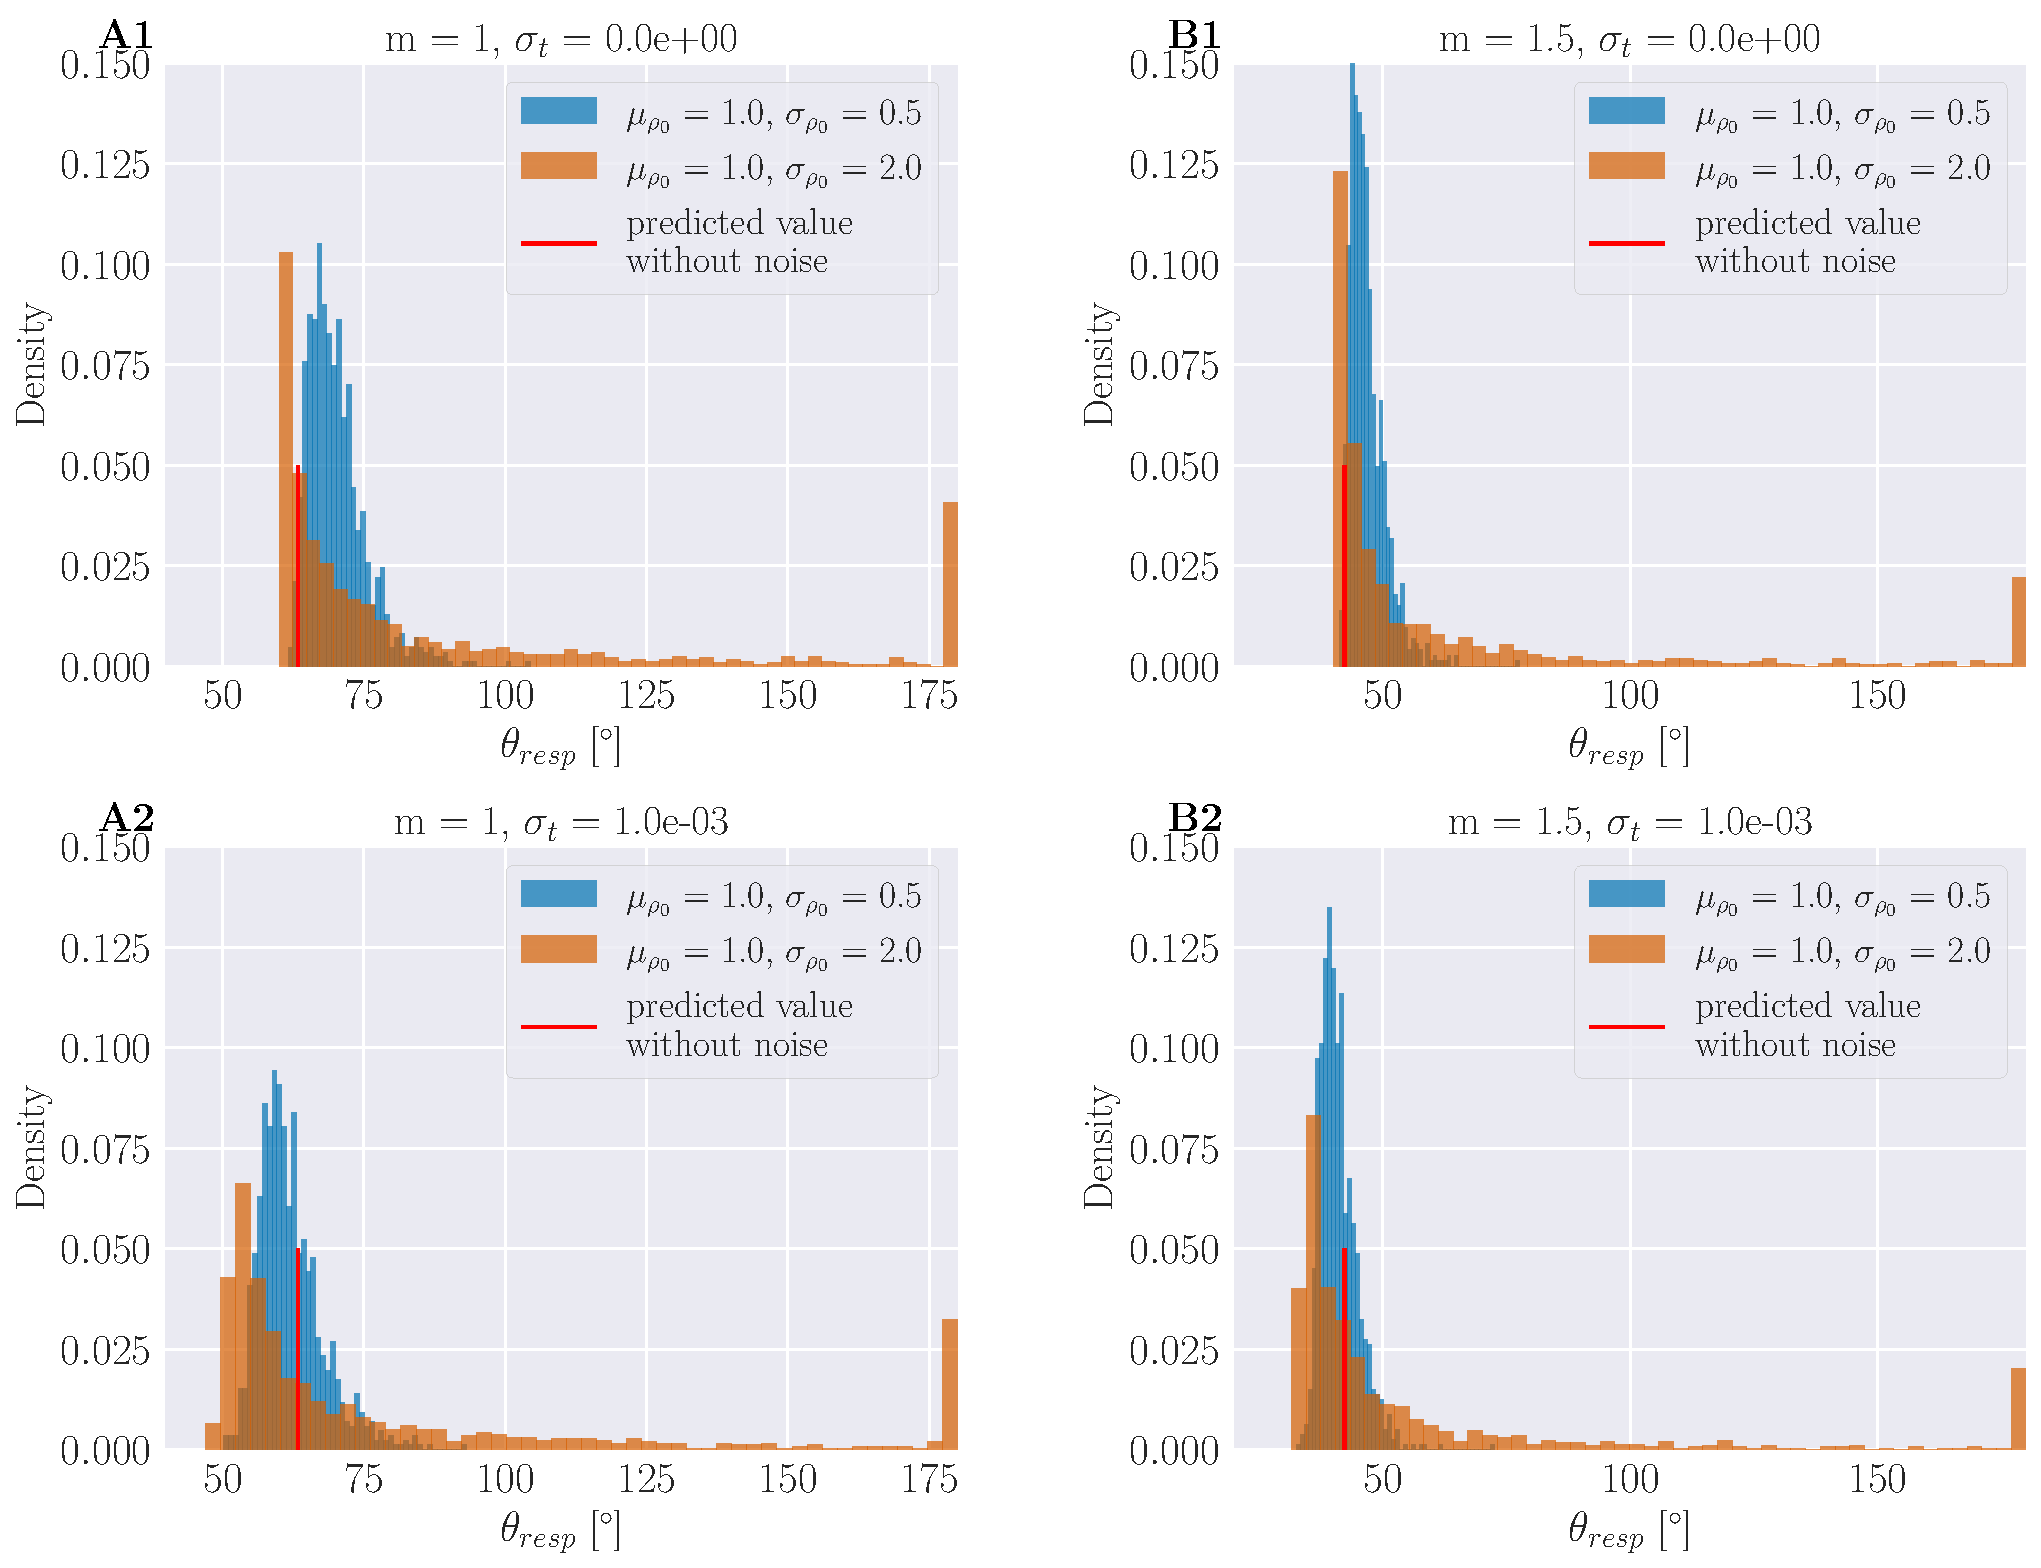
\includegraphics[width=\textwidth]{figure_stationary_rho_null_noise.pdf}
    	\end{center}
    	\caption{\textbf{Response angle distributions for noise of the resting activity of the inhibitory population.} For $b=0$, $c_{scale}=3\cdot10^{-10}$, $c_{\rho}=0.9\cdot 10^{7}$. Sampling the resting activity of the inhibitory population from a log-normal distribution generally increases the response angle. For a small variance the response angle distribution is similar to a Gaussian distribution. Increasing the variance reduces the mode of the distribution but introduces a long tail of higher response angles. The bar at 180 \textdegree{} represents trials for which the M-cell did not fire. These effects are independent of the value of the response angle without noise(\textbf{A} vs. \textbf{B}). Adding threshold noise shifts the distribution towards smaller response angles as observed in Figure \ref{fig:effect_noise_stationary} and minimally changes the shape of the distribution (\textbf{A2} and \textbf{B2}.}
    	\label{fig:effect_rho_null_stationary}
    \end{figure}
    
    \begin{figure}[H]
    	\begin{center}
			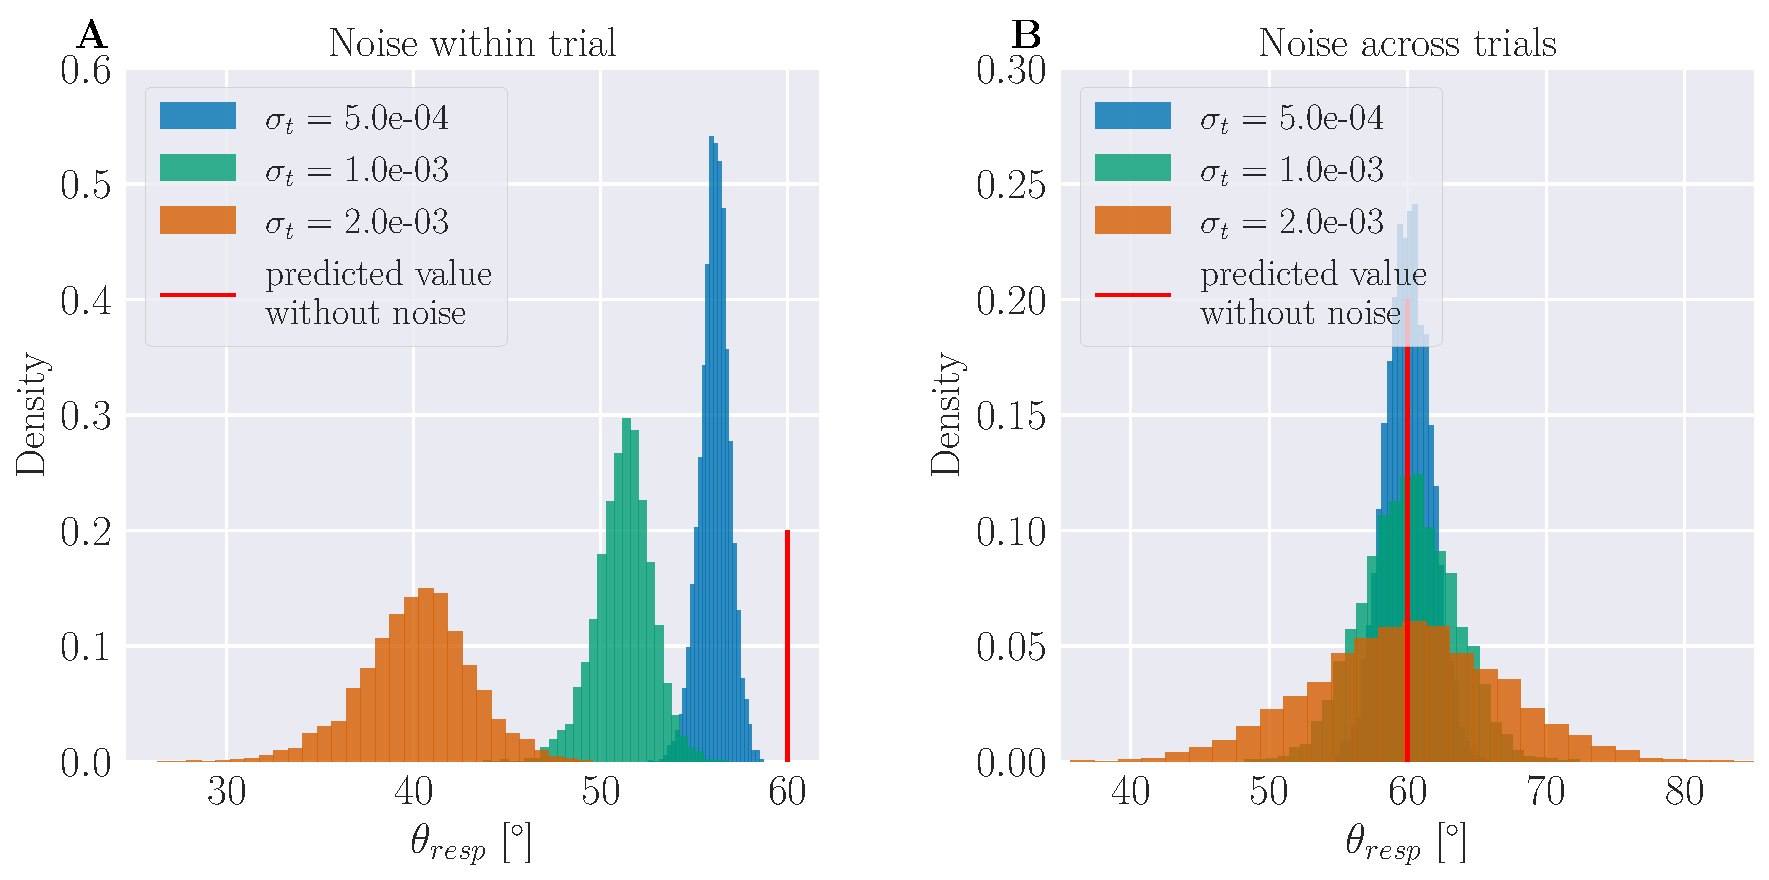
\includegraphics[width=\textwidth, height=0.25\textheight]{figure_static_vs_dynamic_noise.pdf}
    	\end{center}
    	\caption{\textbf{Instantaneous versus constant noise.} While instantaneous noise (\textbf{A}) also decreases the mean response angle, constant noise (\textbf{B}) only affects the variance of the resulting response angle distribution.}
    	\label{fig:static_vs_dynamic_noise}
    \end{figure}

    \section{Stationary approximation of Inhibitory Population}
    In the model of section \ref{approx inhibition}, equation \ref{eq:inhib_approx} we only approximated the activity of the inhibitory population.
    In comparison with the previous section the only difference is that the membrane potential $V_{m}$ now follows the differential equation and thus integrates the input on a time scale that is set by the membrane time constant $\tau_m$ which has been found to be 23 ms in the study of \cite{Koyama2016}.
    For the fastest stimuli (small L/V values) this leads to a deviation from the stationary solution of the previous section (Figure \ref{fig:station_inh_resp_angle}).
    In these cases the response angle is bigger than the response angle predicted by the stationary solution because the input is integrated with a delay so that by the time the membrane potential reaches the threshold, the visual angle already increased beyond the critical value that we would expect from the stationary solution.
    As expected, the deviation increases as the L/V values become smaller (and therefore faster for the same stimulus size).
    The deviation also increases for a bigger $\tau_m$ and decreases for a smaller $\tau_m$, further supporting the notion that the deviation stems from the slower time scale.
        
    \begin{figure}[H]
    	\begin{center}
			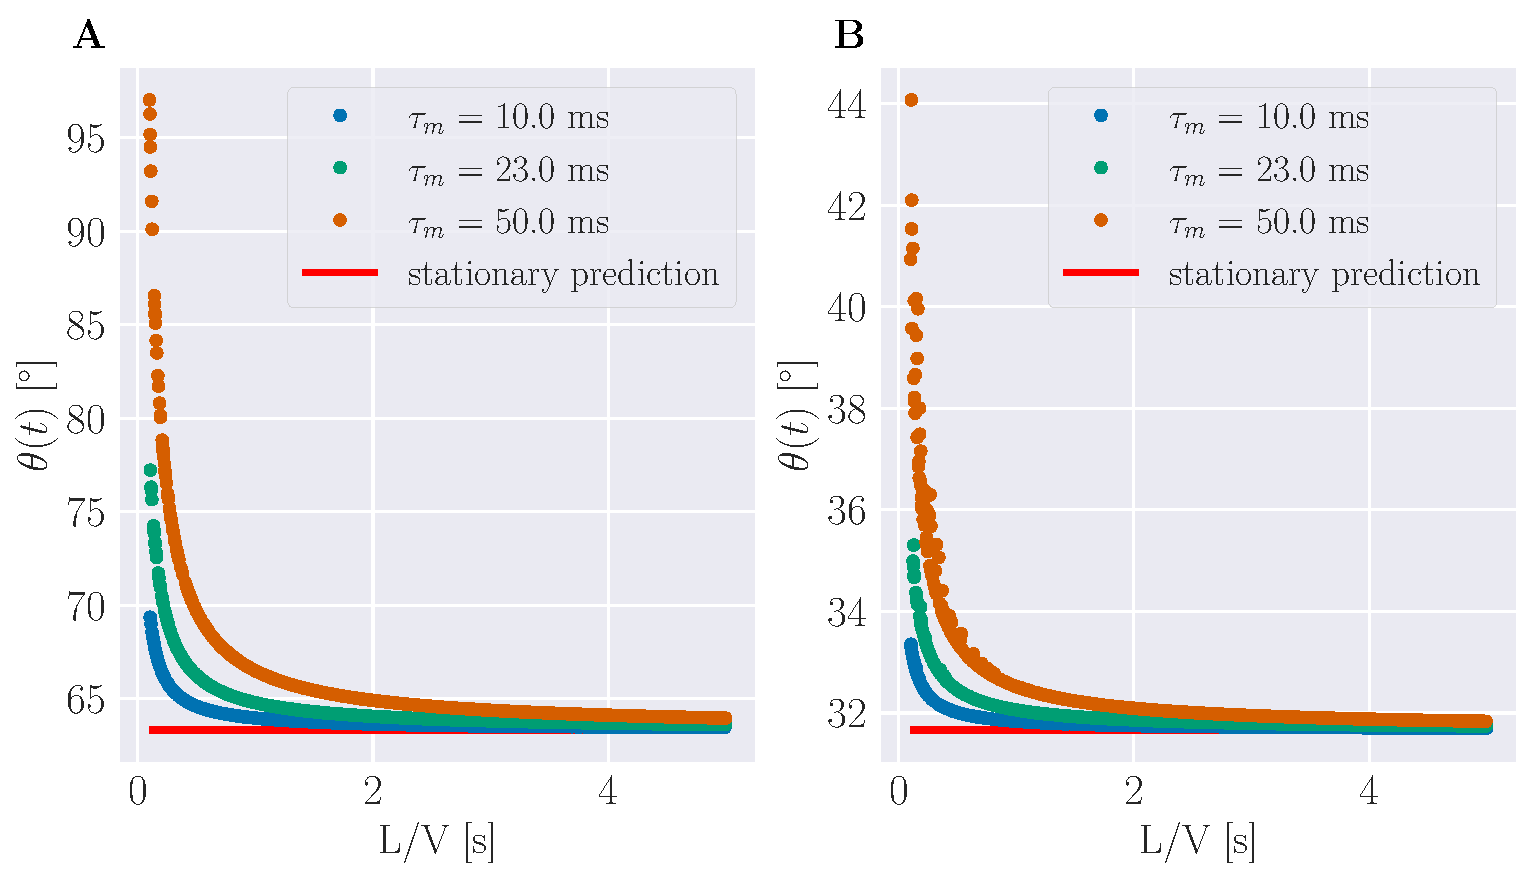
\includegraphics[width=\textwidth]{figure_station_inh_resp_angle.pdf}
    	\end{center}
    	\caption{\textbf{Response angles deviate from stationary solution for fast stimuli.} The response angle for the model with LIF dynamics and a stationary approximation of the inhibitory population activity is plotted against the L/V value of the stimulus using the same range of stimulus sizes L as in \cite{Bhattacharyya2017} (10 - 25 mm) but a larger range of L/V values. For the largest L/V values, the response angle closely matches the fully stationary solution and decreasing L/V leads to higher response angles than the stationary solution with a difference of about 25\% for the smallest L/V value and $\tau_{m}$ = 23 ms in \textbf{A}. Increasing the membrane time constant increases the deviations. The effect holds for different response angle levels (\textbf{A} and \textbf{B}).}
    	\label{fig:station_inh_resp_angle}
    \end{figure}
    
    \section{Full neuronal model}
    Coming back to the full neuronal model as described by equations \ref{eq:inhib}, \ref{eq:mcell} and \ref{eq:thrs} we have now additionally the time scale that the inhibitory population works on.
    This again leads to deviations from the stationary solution but for the inhibitory population the response angle decreases for faster stimuli because the inhibition lacks behind the excitation of the membrane potential.
    Effectively, this results in the same qualitative pattern that we saw in the previous section but with a decreased amount of deviation because the delays from the membrane time constant and the inhibitory population time constant compensate each other partially (compare Figure \ref{fig:full_model_resp_angle} and \ref{fig:station_inh_resp_angle}).
    But this only holds if we set the time constant of the inhibitory population $\tau_{\rho}$ to 1.
    We did this because studies of the auditory pathway suggest that the synapses of the feed-forward inhibition are electrical and therefore operate on a fast time scale.
    As this is not necessarily true for the visual pathway we also analyzed slower time scales for the inhibitory population and find that already for $\tau_{\rho}$ = 5 ms (and fixing $\tau_m$ = 23 ms) the deviation from the stationary response angle flips and we now have smaller response angles (Figure \ref{fig:full_model_effect_tau_inh}).\\
    These differences in the time delays between the different models are illustrated for a single trial with a slow and with a fast stimulus in Figure \ref{fig:voltage_traces}.
    For the slow stimulus (left column) all three model versions show similar voltage traces (bottom row) and therefore result in similar response angles.
    For the fast stimulus (right column) we see that in the full neuronal model the inhibitory input is slightly smaller than in the other two models where the inhibitory population activity is approximated by the stationary solution (blue line vs. green and orange in the second row from the top).
    This leads to a higher total effective input for the M-cell (blue line is higher in the third row from the top) and thus the membrane potential reaches the firing threshold earlier (bottom row) which means that the response angle is smaller than in the other two models (first row).
    On the other hand, for the stationary inhibition model the effective input for the M-cell is the same as in the fully stationary model (green and orange lines in the third row from the top) but due to the LIF dynamics with the membrane time constant the input is integrated with a delay so that the membrane voltage reaches the threshold later (bottom row) and thus the response angle is higher (top row).
    \begin{figure}[H]
    	\begin{center}
			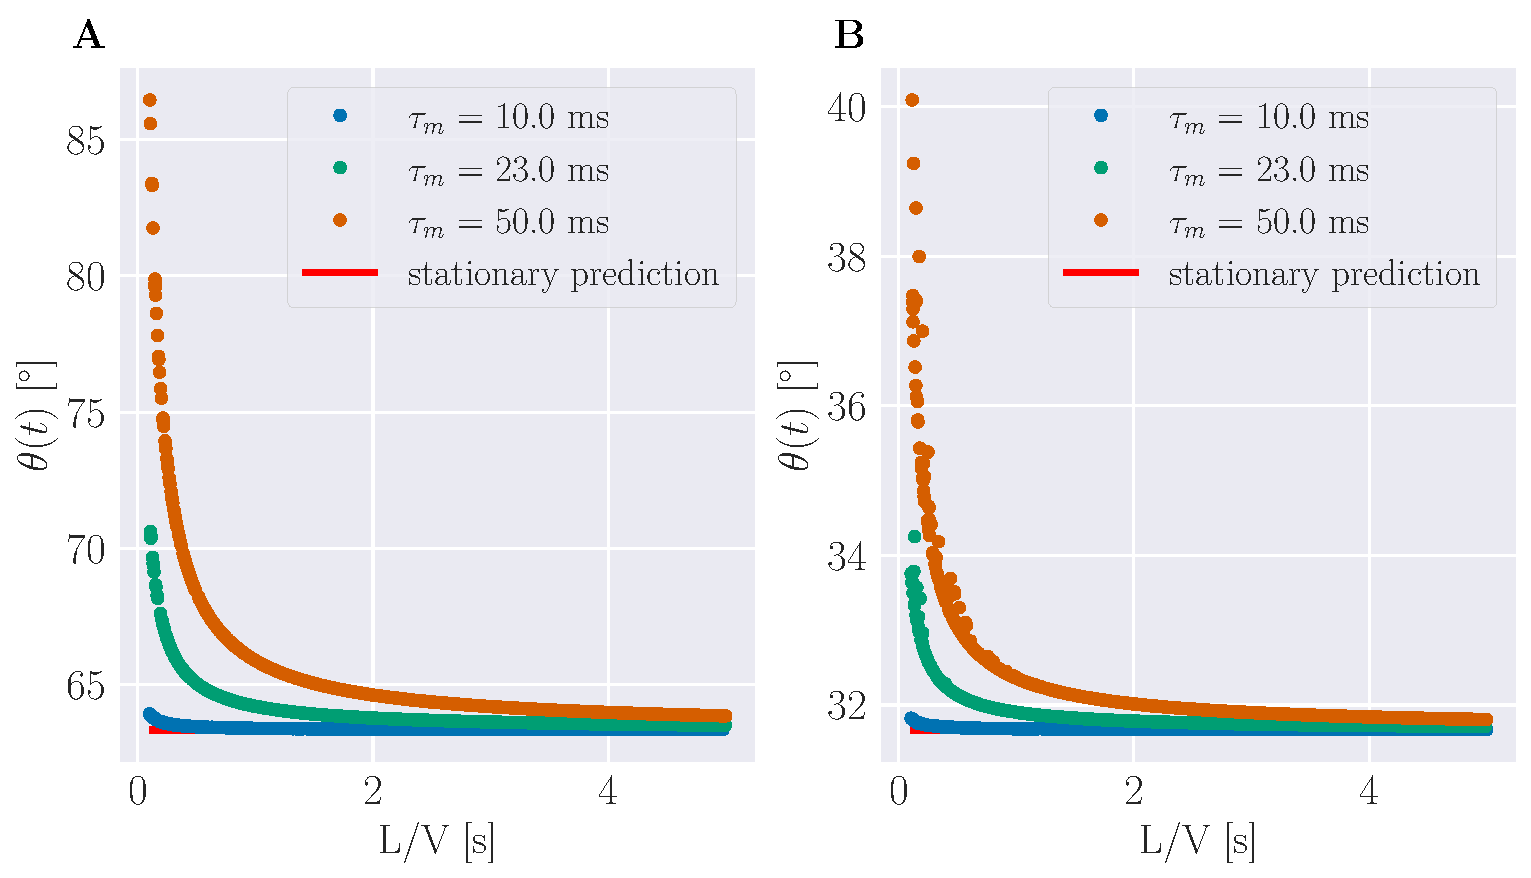
\includegraphics[width=\textwidth]{figure_full_model_resp_angle.pdf}
    	\end{center}
    	\caption{\textbf{Full model response angles deviate less from stationary solution.} The response angle for the full neuronal model is plotted against the L/V value of the stimulus using the same range of stimulus sizes L as in \cite{Bhattacharyya2017} (10 - 25 mm) but a larger range of L/V values. We see the same qualitative pattern as in Figure \ref{fig:station_inh_resp_angle} but here the deviations are less pronounced with a difference of only about 10\% for the smallest L/V value and $\tau_{m}$ = 23 ms in \textbf{A}. Increasing the membrane time constant increases the deviations. The effect holds for different response angle levels (\textbf{A} and \textbf{B}).}
    	\label{fig:full_model_resp_angle}
    \end{figure}
    
    \begin{figure}[H]
    	\begin{center}
			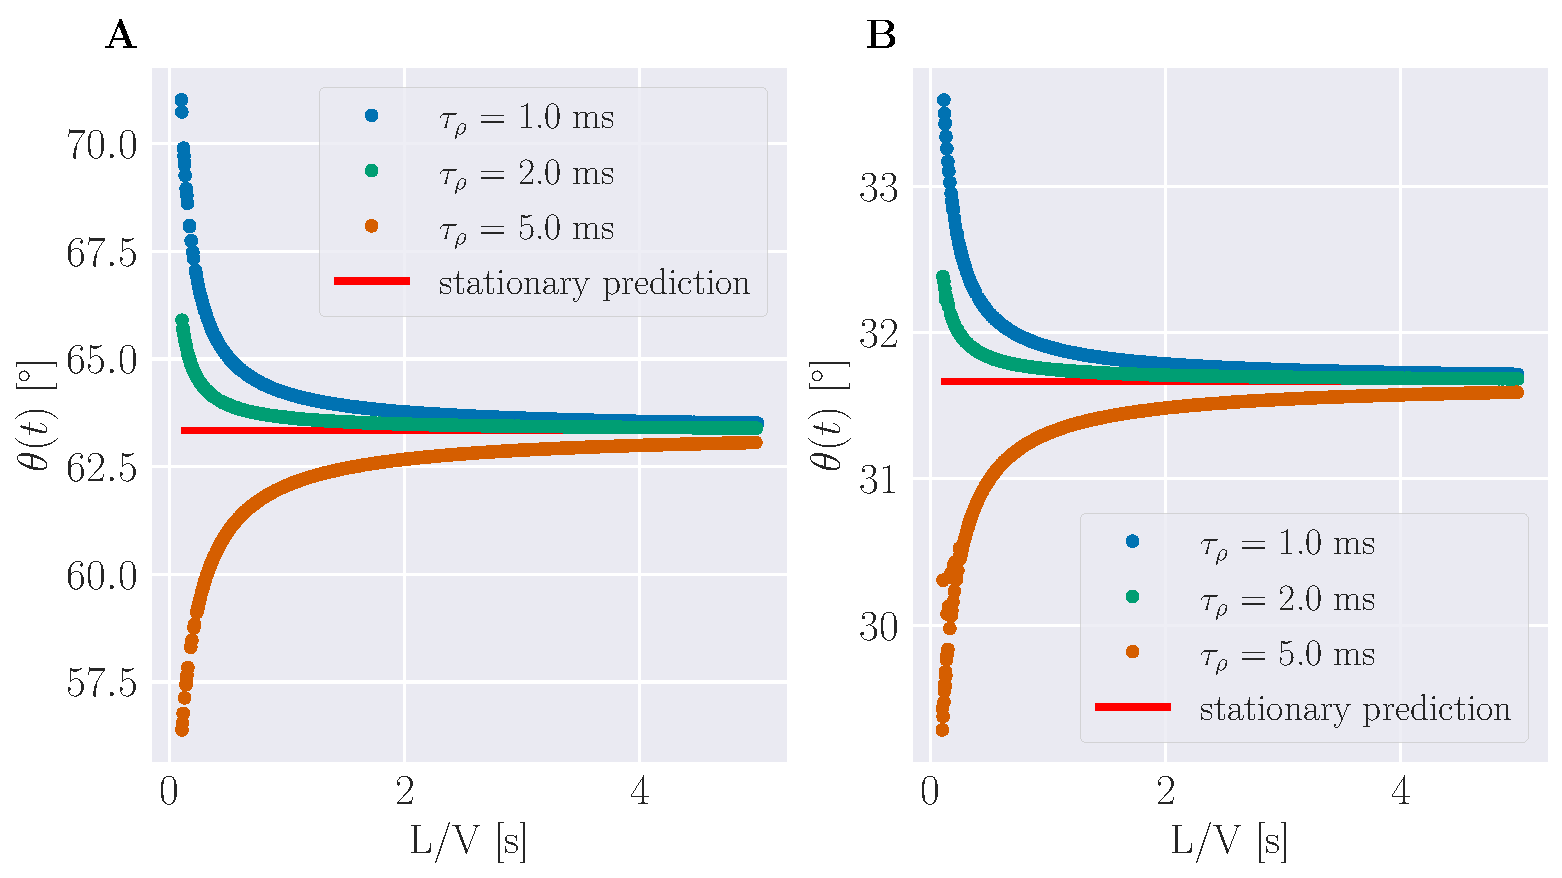
\includegraphics[width=\textwidth]{figure_full_model_resp_angle_tau_inh.pdf}
    	\end{center}
    	\caption{\textbf{Higher inhibitory time constants decrease the response angle.} Same setup as in Figure \ref{fig:full_model_resp_angle} but with $\tau_m$ = 23 ms and variable $\tau_{\rho}$. Increasing $\tau_{\rho}$ leads to lower response angles and at $\tau_{\rho}$ = 5 ms to response angles that are lower than the stationary solution. The effect holds for different response angle levels (\textbf{A} and \textbf{B}).}
    	\label{fig:full_model_effect_tau_inh}
    \end{figure}
    
     \begin{figure}[H]
    	\begin{center}
			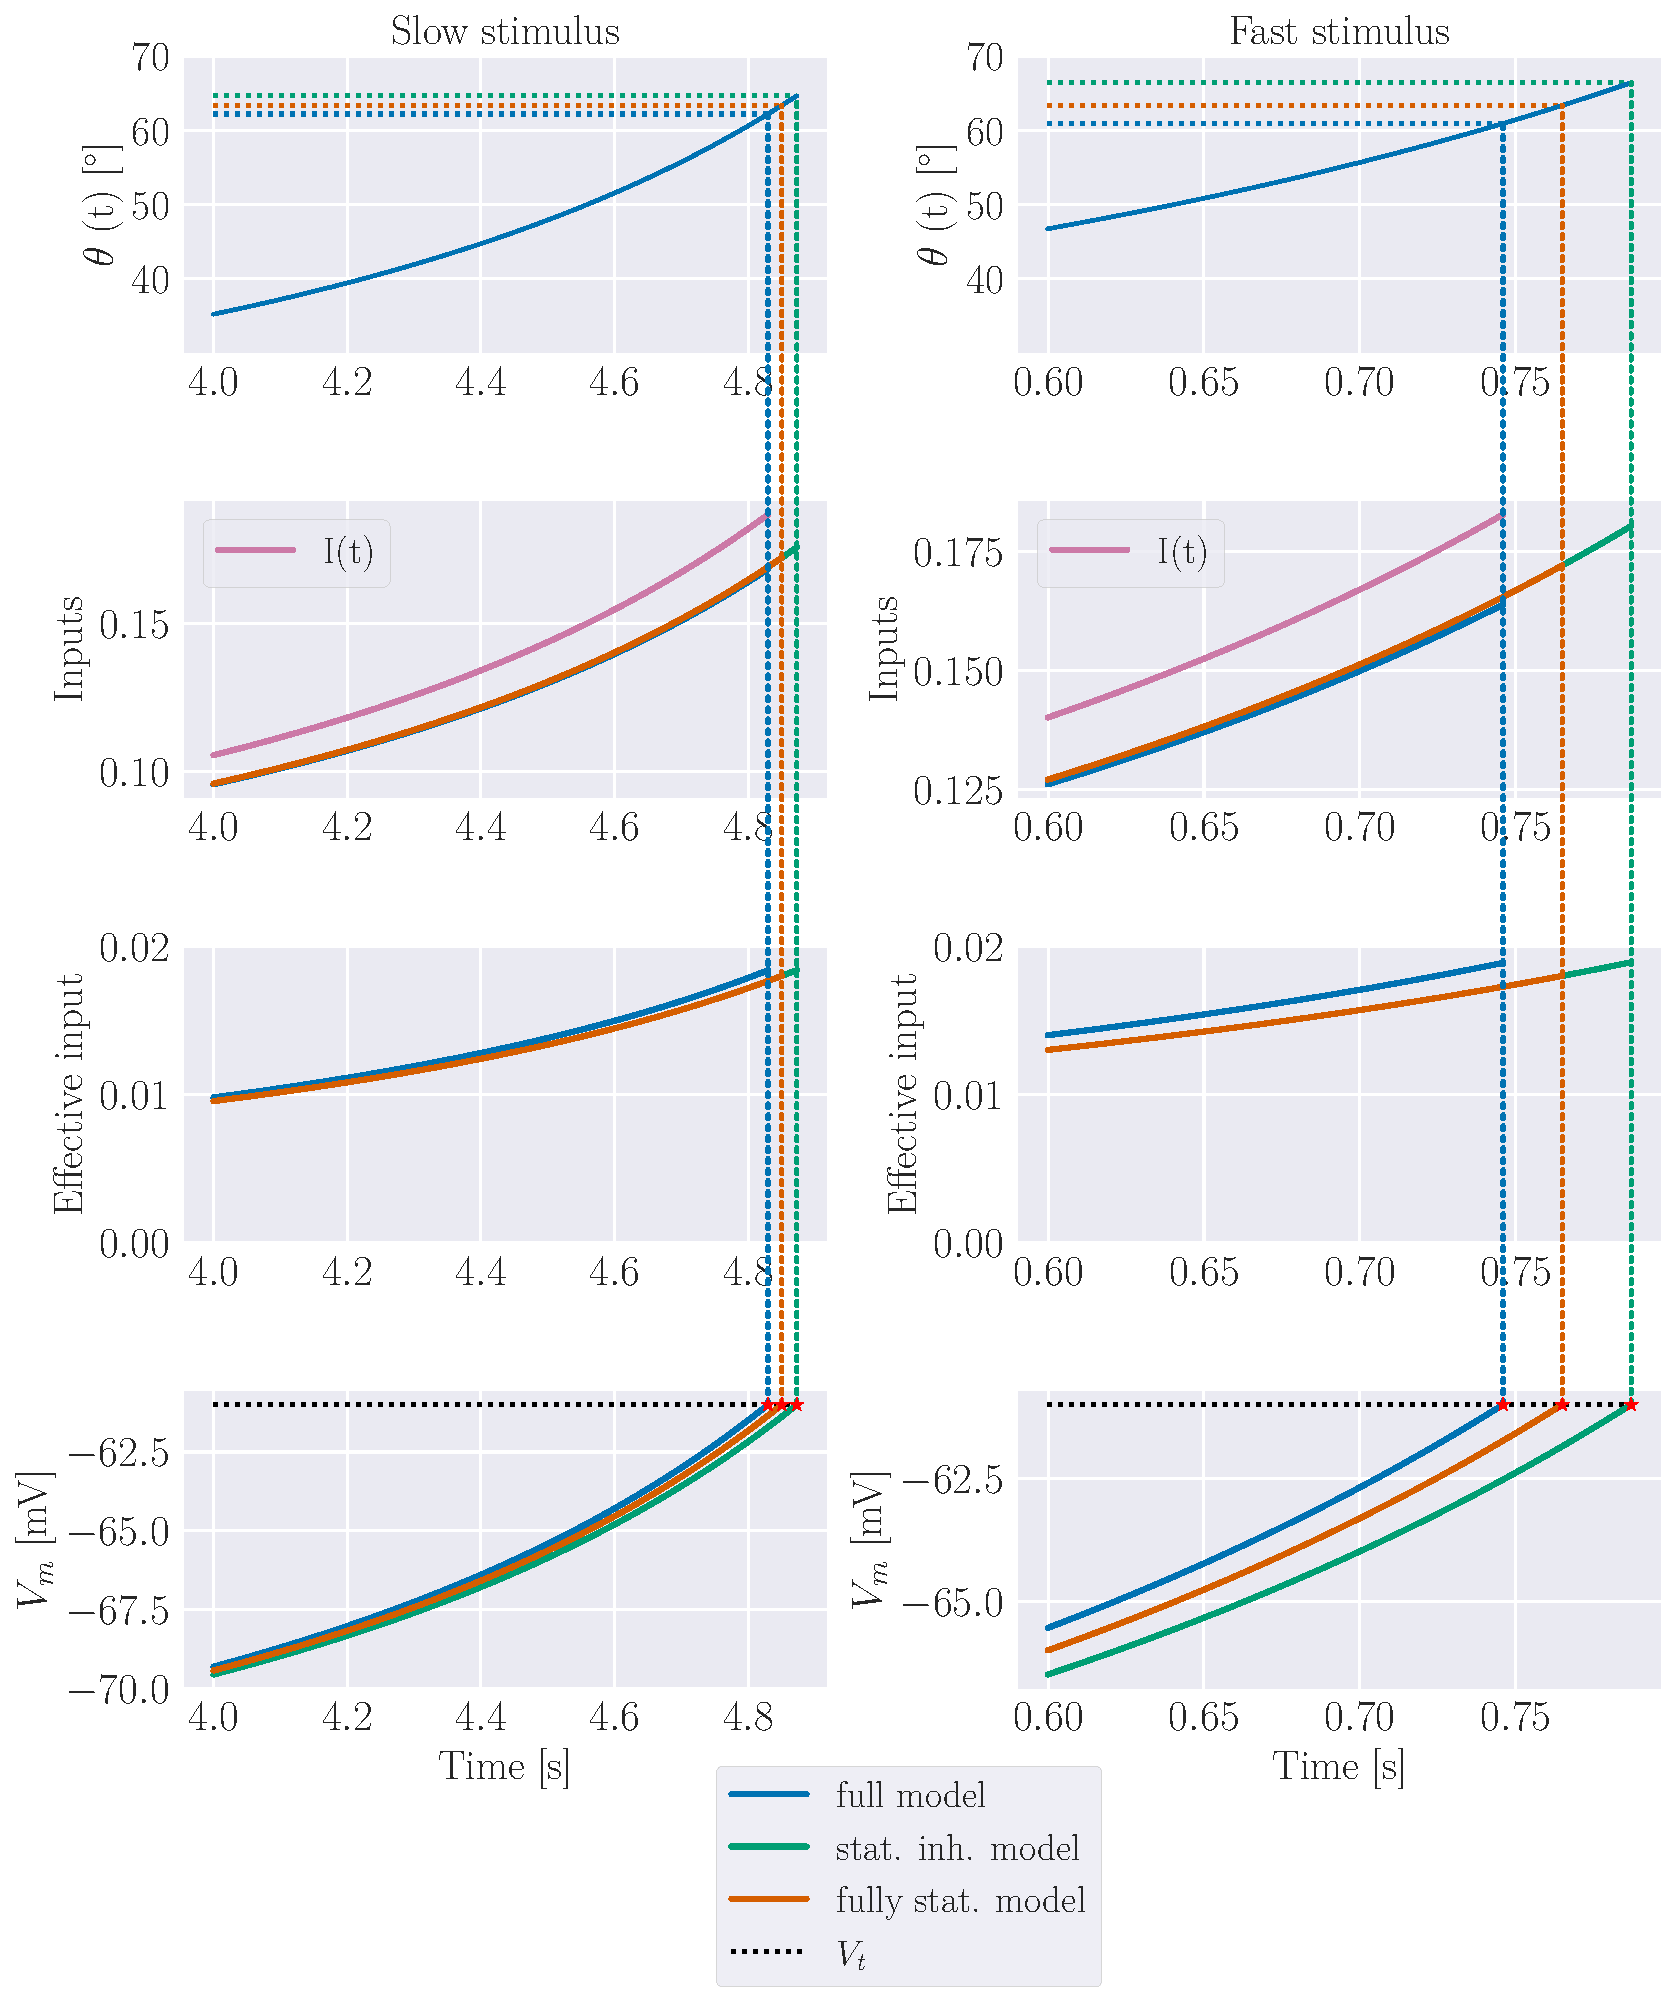
\includegraphics[width=\textwidth]{figure_voltage_traces.pdf}
    	\end{center}
    	\caption{\textbf{Single trial comparison of the different models for a slow and a fast stimulus.} Each of the two columns shows from top to bottom 1) the visual angle of the stimulus, 2) the excitatory and the inhibitory input for the M-cell, 3) the effective input for the M-cell and 4) the membrane voltage of the M-cell. While the models show very similar traces for the slow stimulus (left column), a fast stimulus leads to bigger differences in the resulting response angle.}
        %TODO: edit caption
    	\label{fig:voltage_traces}
    \end{figure}
    
    \section{Parameter fitting}
    In order to find out which parameter values account best for the observed response angles we fitted the full neuronal model to the data of \cite{Bhattacharyya2017} (see Figure \ref{fig:expm_theta_lv}).
    We used only this dataset because we have the response angles and the sampled L/V values for all trials instead of only the mean values of the response angle.
    Furthermore, since the study was done with zebrafish, we could use the fitted parameter values from \cite{Koyama2016} to constraint the model.\\
    For the fitting, we used the recently published library \textit{Delfi}, developed by \cite{Lueckmann2018}.
    The library implements several inference algorithms, from which we used the Sequential Neural Posterior Estimation (SNPE).
    Briefly, the algorithm uses a Mixture-Density Network (MDN) as a density estimator that approximates the true posterior distribution of the model parameters given the observed data.
    This is achieved by sequentially training the parameters of the MDN with data that is generated by the model using model parameters that are sampled from the current prior distribution.
    After such a training round the prior is updated to be the current estimated posterior distribution and this is repeated until the estimated posterior converges to the true posterior which can be evaluated by the importance-weighted log loss.
    For further details see \cite{Lueckmann2018} and the documentation of \textit{Delfi} (version 0.4.1) at \href{http://www.mackelab.org/delfi/}{http://www.mackelab.org/delfi/}.\\
    The parameters of the algorithm consist of the number of hidden layers of the neuronal network, the number of neurons for each layer, the number of rounds, the number of training trials for each round and the number training epochs.
    Here we used three hidden layers with 330 neurons each and trained for a single round of 40000 training trials with 100 epochs.\\
    In order to efficiently learn the mapping between the data and the posterior distribution we reduced the dimensionality of the raw data, which consisted of pairs of L/V values and response angles for 246 trials, by computing five quantile values (10\%, 30\%, 50\%, 70\% and 90\%) of the response angles in six bins for the L/V values resulting in 30 data points.
    How this reduction looks like for the data of \cite{Bhattacharyya2017} is shown in Figure \ref{fig:expm_data_to_quantiles}.\\
    \begin{figure}[H]
    	\begin{center}
			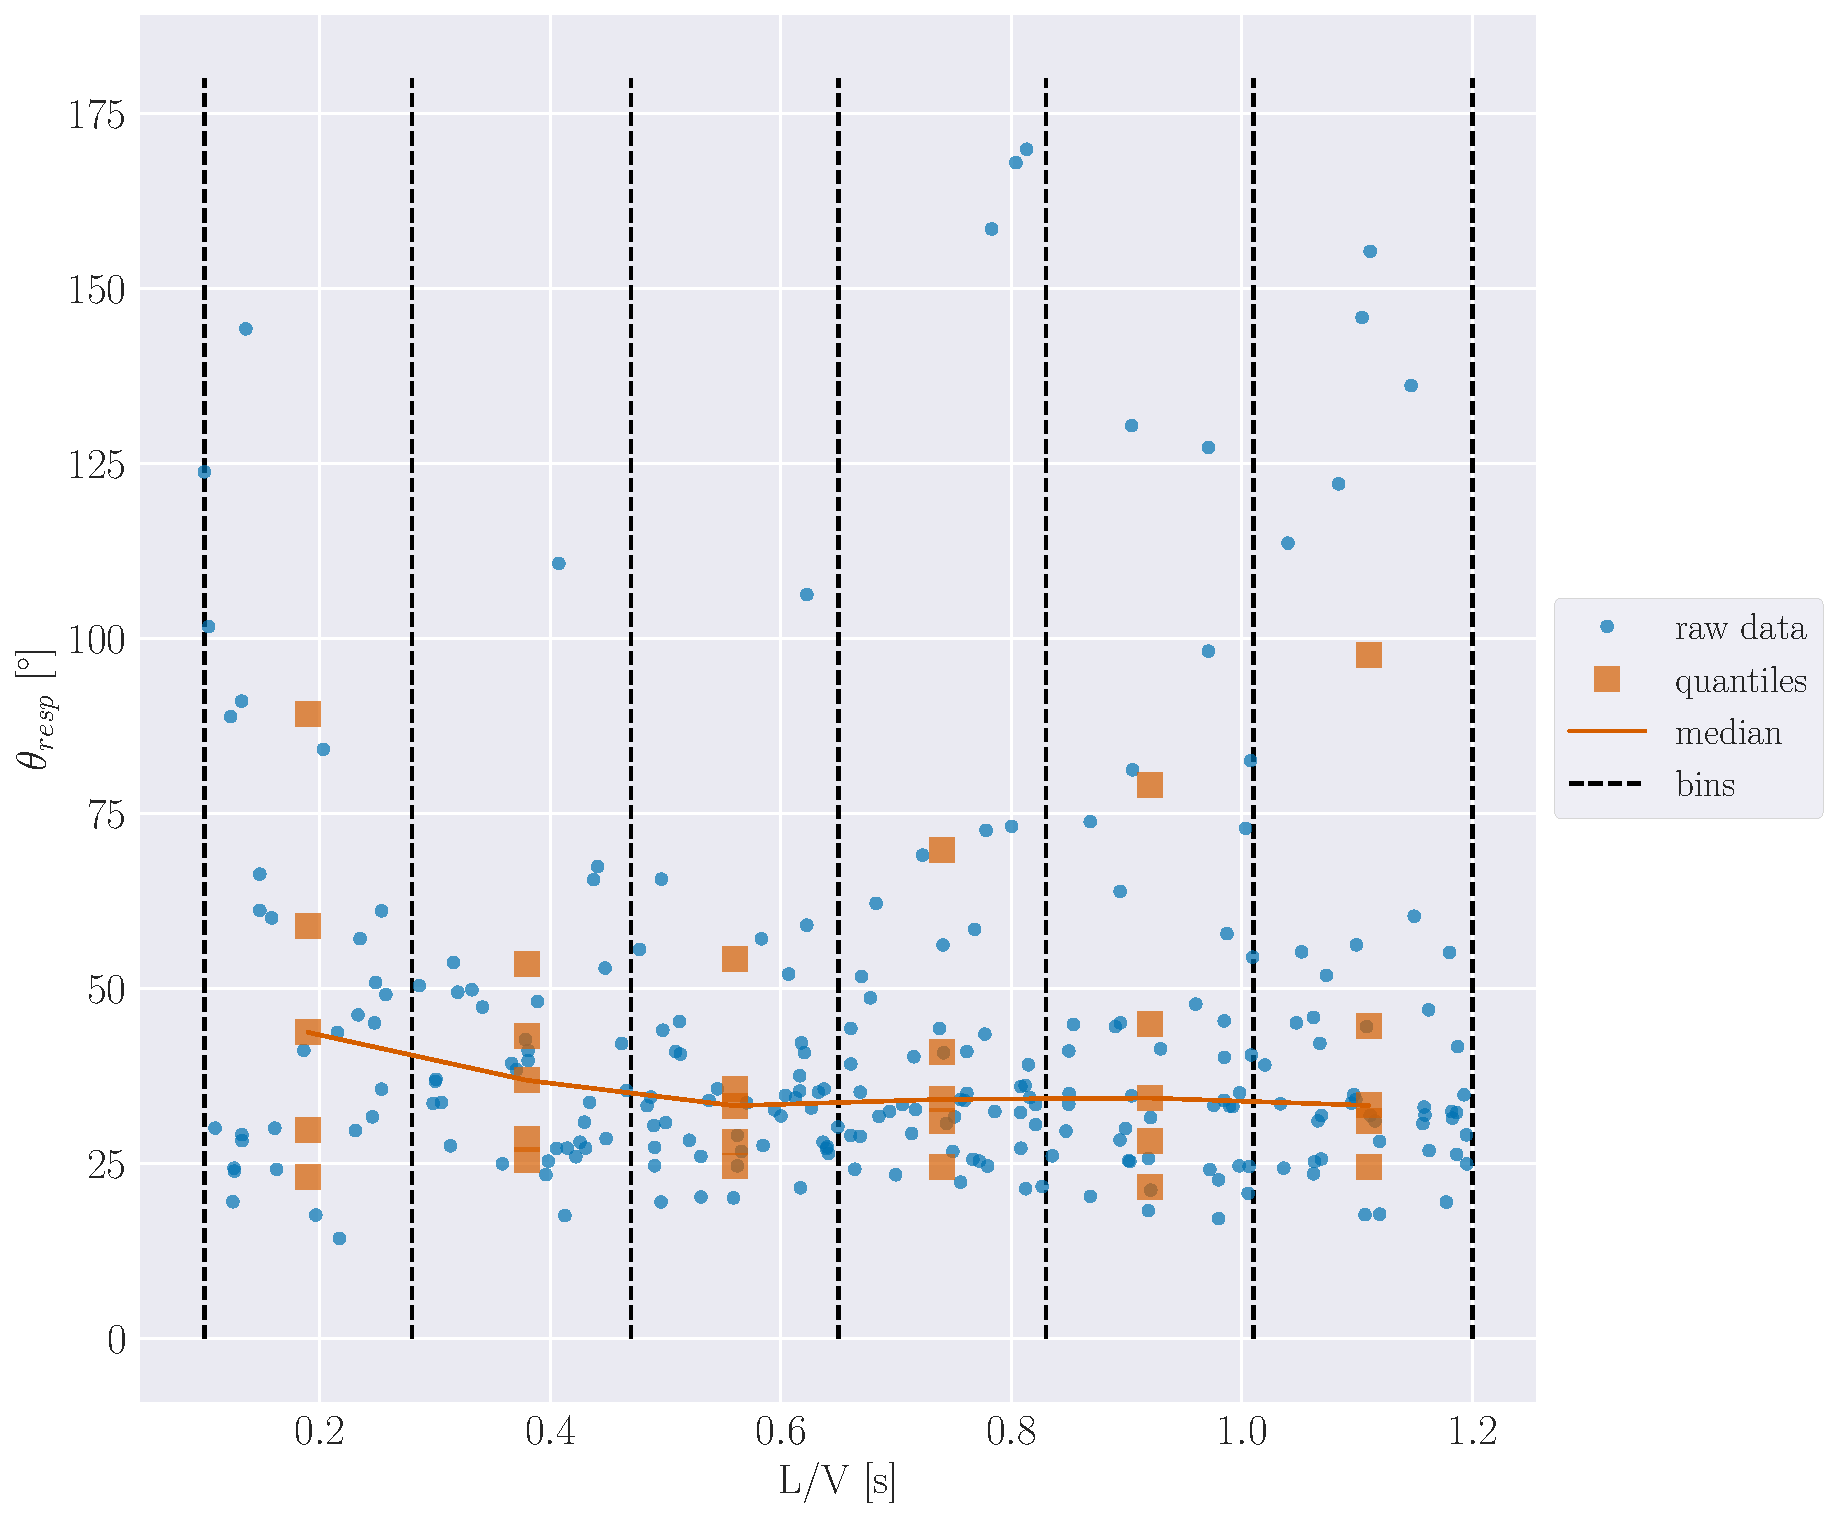
\includegraphics[width=\textwidth]{figure_data_to_quant.pdf}
    	\end{center}
    	\caption{\textbf{Data summary statistic for the fitting algorithm.} The range of L/V values (0.1 to 1.2) is divided in 6 bins and for each bin the 10\%, 30\%, 50\%, 70\% and 90\% quantiles are computed. The resulting quantile values are shown for the dataset of \cite{Bhattacharyya2017}.}
    	\label{fig:expm_data_to_quantiles}
    \end{figure}
    Out of the remaining 14 parameters after fixing the electrophysiological parameters of the M-cell at the values from \cite{Koyama2016}, we only fitted $\mu_{\rho_{0}}$, $\sigma_{\rho_{0}}$, $c_{\rho}$, and $\eta_{m}$.
    The remaining parameters are the trial time, the initial resting time, the simulation time step, the input scaling factor, the noise variances for the firing threshold and the inhibitory population, the time constant of the inhibitory population, the slope and offset of the linear transformation of the input and finally the cutoff angle.
    We fixed to 5 s and 2 s, resembling the corresponding times in the experiment.
    The simulation time step was set to 1 ms, which is enough to capture all relevant dynamics in the simulation.
    Setting the input scaling to $3 \cdot 10^{-10}$, the slope of the linear transformation to 3 and the offset to zero sets the baseline response angle to a medium value.
    We used a cutoff angle of 180\textdegree{} which is the maximal visual angle that is physically possible.
    We further assume a reasonable amount of noise with a standard deviation of 5 mV on the activation of the inhibitory population and set the time constant for the inhibitory population to 1 ms motivated by electrical synapses as described before.\\
    Since the algorithm uses Bayesian inference we need to define priors for the parameters that we want to fit.
    We chose uniform distributions for all parameters and the ranges were generally choses such that the model can result in very different patterns of response angle distributions but not too extreme.
    For the two parameters of the distribution of $\rho_0$ we chose the ranges 0 to 5 and 0.5 to 5 for the mean and variance respectively.
    This allows for for almost normally distributed values if both parameters are small or very skewed distributions if the variance is higher (see also Figure \ref{fig:effect_rho_null_stationary}).
    The range for the noise of the membrane potential is 0 to 5 which allows for practically no noise to very noise membrane potential traces.
    Finally, the prior for the inhibitory input scaling $c_{\rho}$ is a uniform distribution that goes from $5\cdot 10^{6}$ to $10\cdot 10^{6}$ where $5\cdot 10^{6}$ would correspond to very weak feed-forward inhibition and $10\cdot 10^6$ would mean that the inhibition fully compensates the excitation from the input.
    An overview of the fixed parameter values, the free parameters and their priors is given in Table \ref{tab:neuroparams}.\\
    As a first step we analyzed how well the fitting procedure would perform on model-generated data.
    We find that the algorithm performance differs between the model parameters but the overall performance is reasonable.
    On a positive note, the fitting results seem to be rather robust since the repetitions that we ran for each ground truth parameter set led to very similar fitted distributions (see the similarity between line "pairs" in each subplot in Figure \ref{fig:fit_validation}).
    The worst result among the single parameters is found for the variance of the membrane noise $\sigma_m$ where the fitted posterior means have all similar values regardless of the true parameter value and also high variances, indicating high probabilities for a wide range of values for $\sigma_m$ (Figure \ref{fig:fit_validation} D).
    For the mean of the distribution for $\rho_{0}$ the true values mostly lie within the standard deviation of the posterior distribution although here as well, the variances of the posteriors are rather high (Figure \ref{fig:fit_validation} A).
    The results for the variance of he distribution for $\rho_0$ are mixed.
    In two cases the posterior means almost perfectly match the true values but in three other cases the true values are underestimated by the posterior (Figure \ref{fig:fit_validation} B).
    Similarly, for the scaling factor of the input for the inhibitory population $c_{\rho}$, the posterior matches the true values rather good in two to three cases but deviates from the true value in the remaining cases (Figure \ref{fig:fit_validation} C).\\
    \begin{figure}[H]
    	\begin{center}
			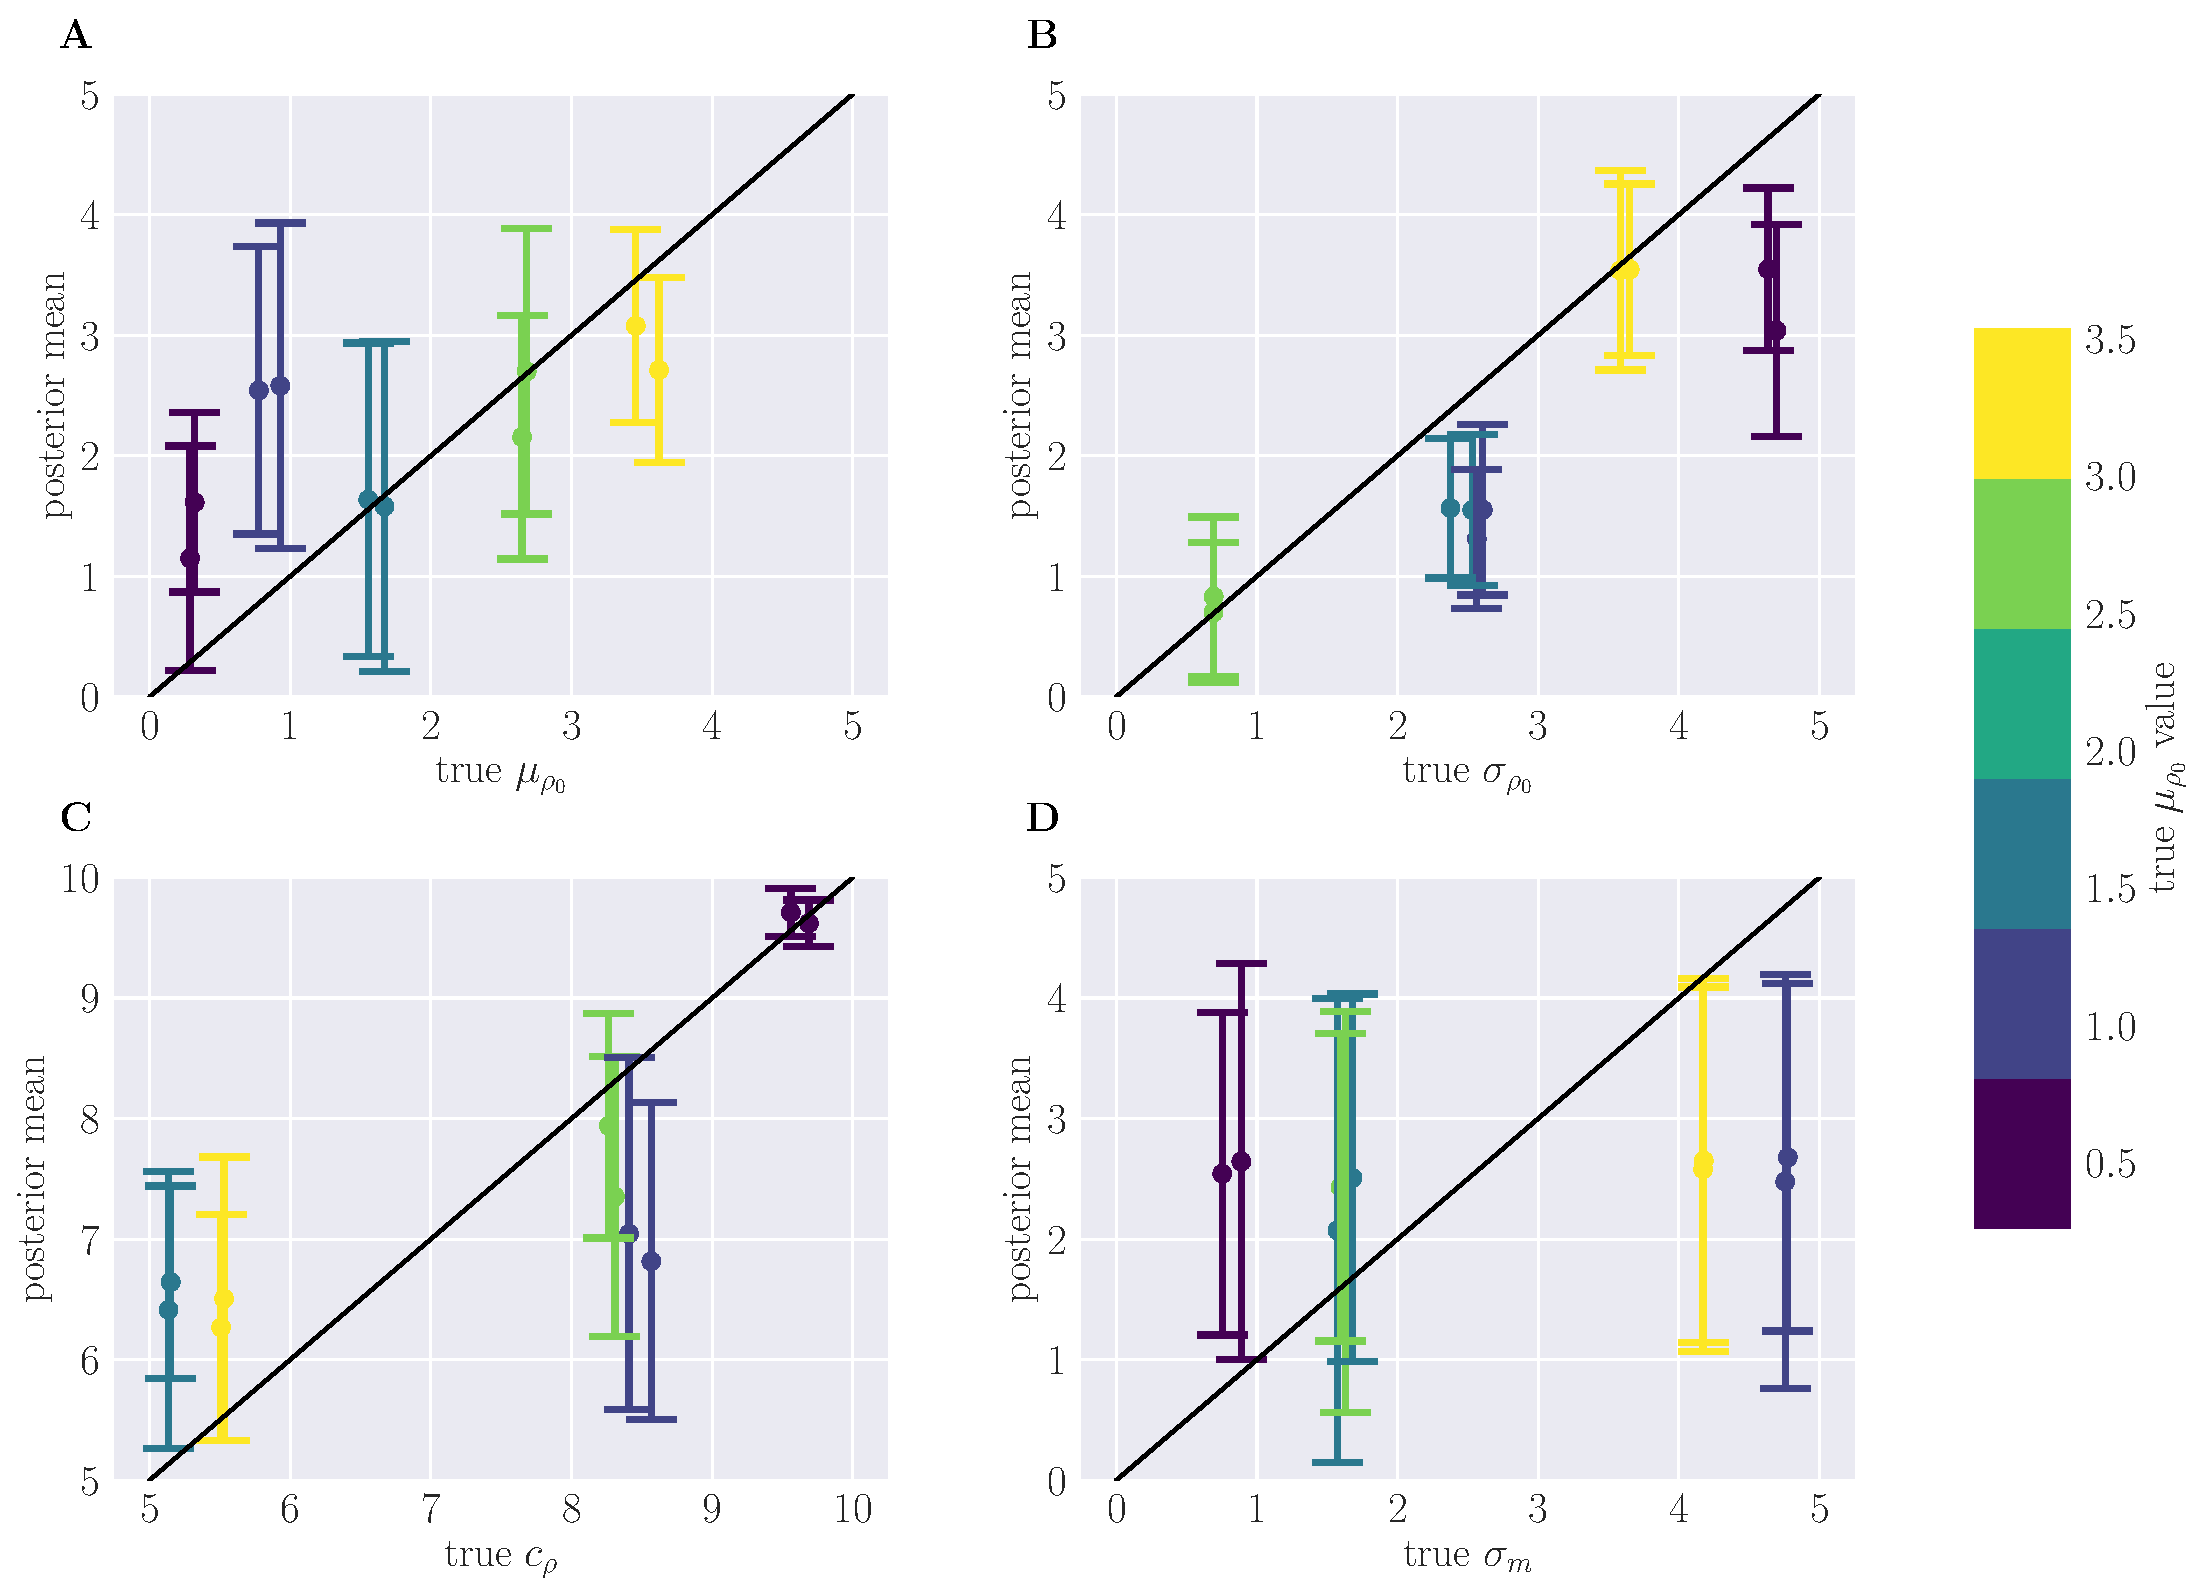
\includegraphics[width=\textwidth]{figure_fit_validation.pdf}
    	\end{center}
    	\caption{\textbf{Validation of fitting procedure.} For datasets that were generated by the model itself the posterior mean and standard deviation after fitting are shown. The posteriors have in general large variances. The parameters $\mu_{\rho_{0}}$, $\sigma_{\rho_{0}}$ and $c_{\rho}$ show the right tendency where larger true values correspond with larger posterior means. The fitted posteriors for the parameter $\sigma_{m}$ have all very similar mean values indicating that this parameter is not recoverable with the current parameter setting of the fitting procedure.}
    	\label{fig:fit_validation}
    \end{figure}
    In the next step we fitted the full neuronal model to the experimental data from \cite{Bhattacharyya2017}.
    The posterior distribution of the fit is shown in Figure \ref{fig:fit_expm_post}.
    As we have already seen in the parameter recovery from above, the posterior mean for the variance of the membrane noise lies in the middle of the prior range and has a high variance.
    This indicates that the exact value of $\sigma_m$ has no big influence on the resulting distribution of data.
    For the remaining parameters we find a rather narrow peak at $\mu_{\rho_0}$ = 3.6, $\sigma_{\rho_0}$ = 0.8 and $c_{\rho}$ = 8.2.
    How the data from the model with these fitted parameters compares to the experimental data is shown in Figure \ref{fig:fit_expm_comparison}.
    If we compare data for the same amount of trials as in the experiment we see a good match, especially for the lower range of response angles (Figure \ref{fig:fit_expm_comparison} A) whereas the model seems to have a higher density of response angles above 60\textdegree{} than in the experiment which is also reflected by the higher deviations for the 90\% quantiles in Figure \ref{fig:fit_expm_comparison} B.
    The higher accuracy for the lower range of response angles makes sense because there are more data points in this range so that the summary statistics are more informed in this range.
    \begin{figure}[H]
    \begin{center}
    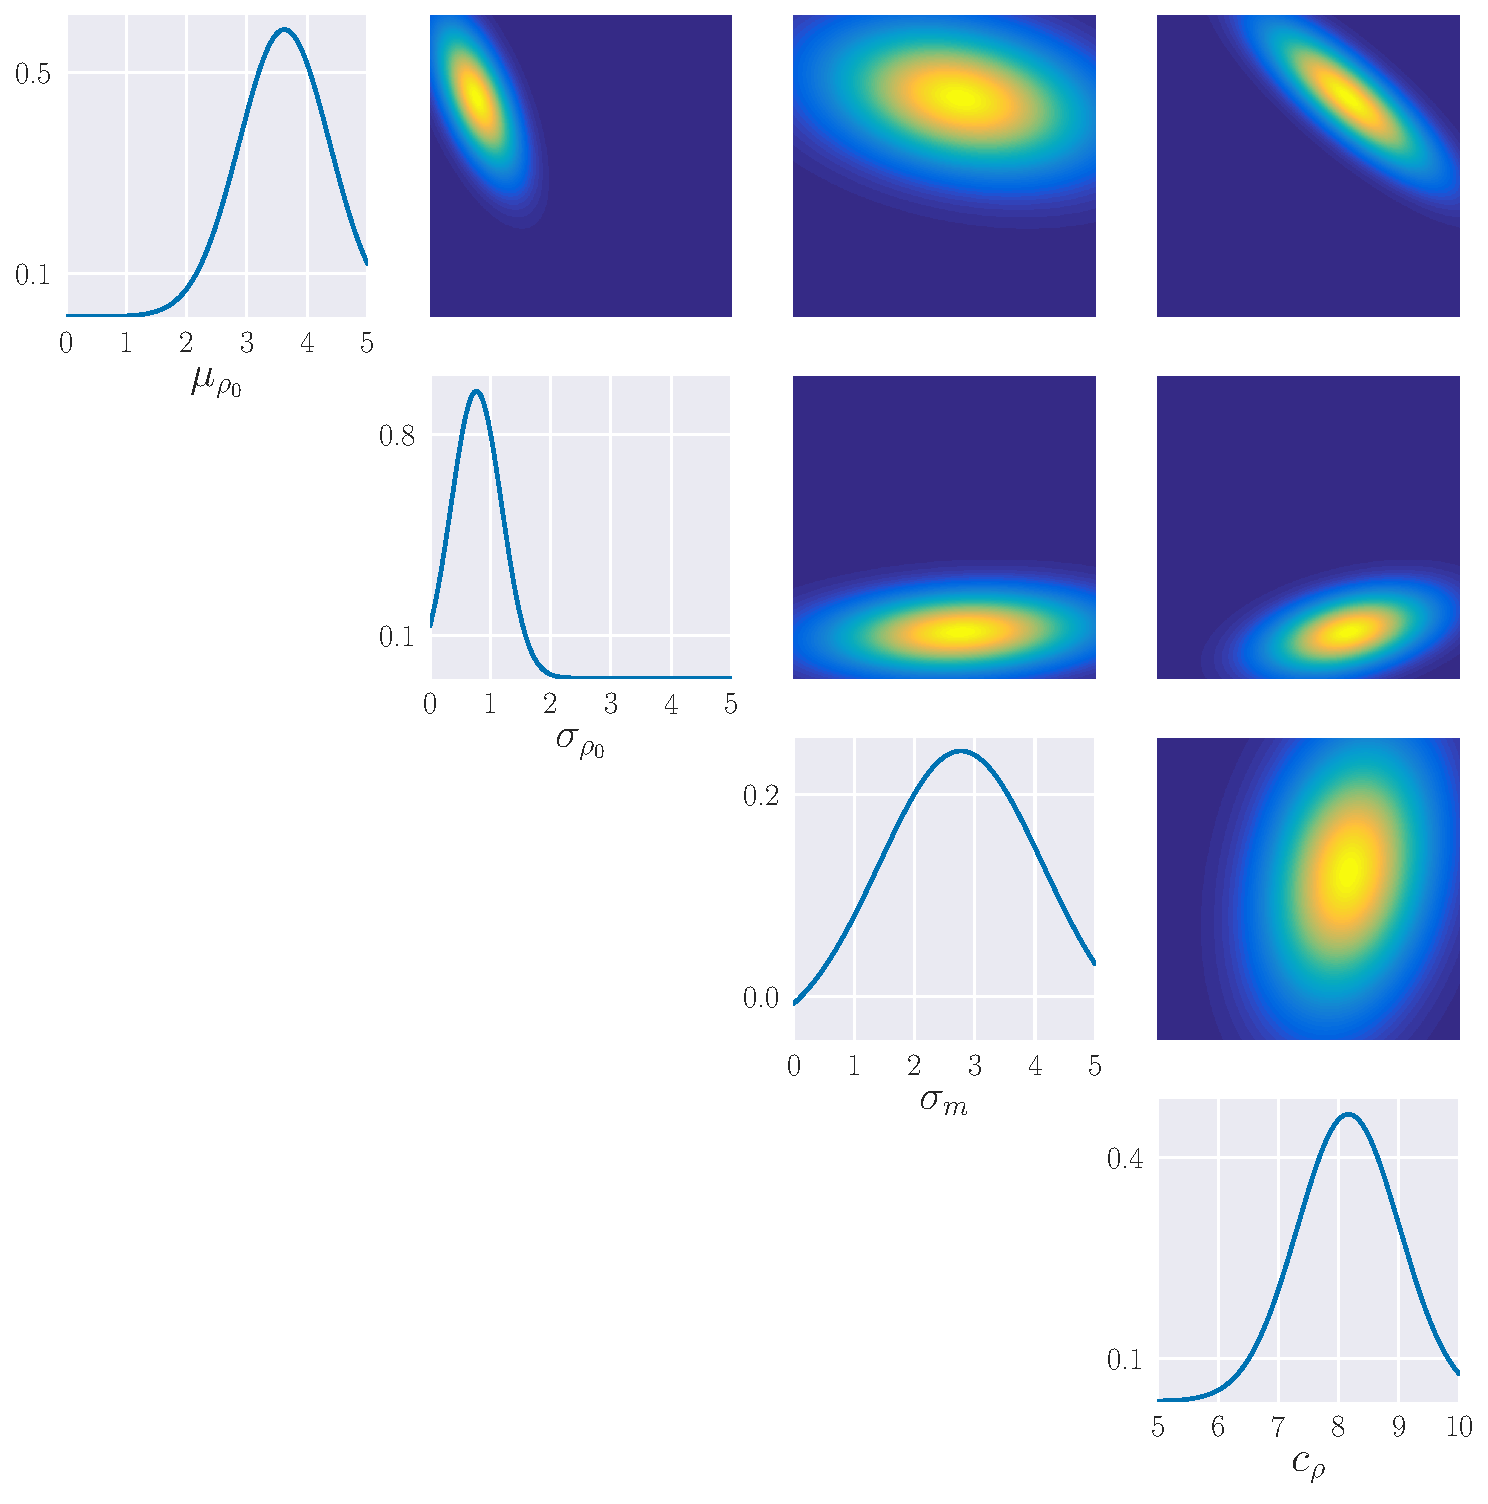
\includegraphics[width=\textwidth]{figure_expm_fit_posterior.pdf}
    \end{center}
    \caption{\textbf{The posterior distribution of the fitted parameters.} The distribution of $\sigma_{\rho_0}$ is the most narrow, indicating high certainty of the fitted mean value. In contrast, $\sigma_{m}$ has much wider distribution, speaking for little influence on the resulting fit. The covariances between $\mu_{\rho_0}$ on the one hand and $\sigma_{\rho_0}$ and $c_{\rho}$ on the other hand show negative correlations, i.e. for smaller values of $\mu_{\rho_0}$ it is more likely for $\sigma_{\rho_0}$ and $c_{\rho}$ to have higher values.}
    \label{fig:fit_expm_post}
    \end{figure}
    
    \begin{figure}[H]
    \begin{center}
    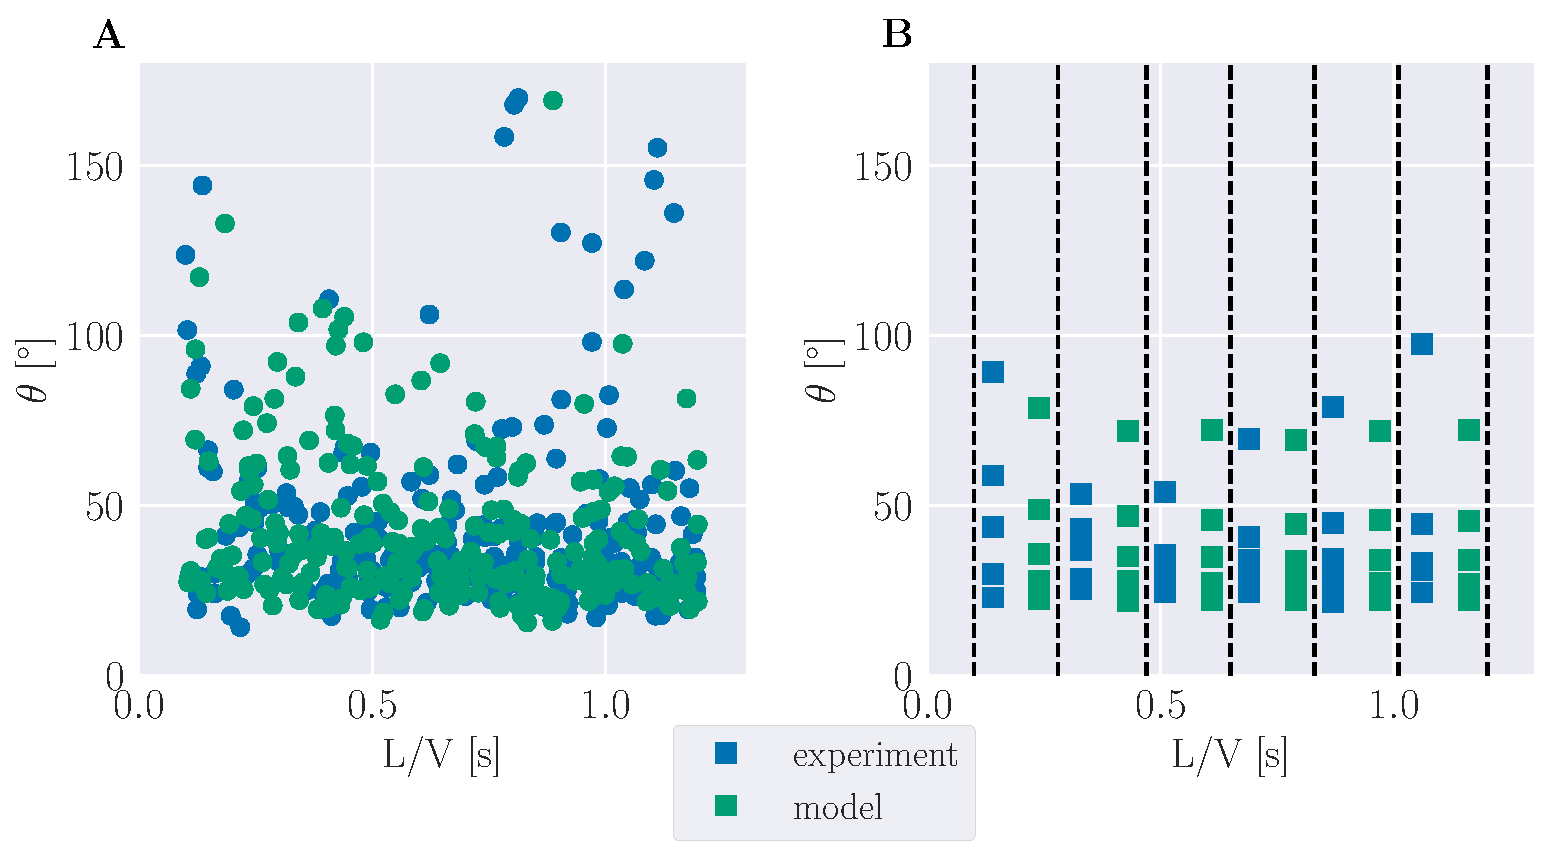
\includegraphics[width=\textwidth]{figure_expm_fit_comparison.pdf}
    \end{center}
    \caption{\textbf{Comparison of experimental data with data generated from the fitted model.} \textbf{A} Response angle data from \cite{Bhattacharyya2017} in blue and data from the same amount of trials generated by the fitted model in green are shown. While the two closely match for the lower range of response angles (20\textdegree{} - 60\textdegree{}), the model seems to generate more response angles in the range of 60\textdegree{} to 100\textdegree{} although this could look very different for different set of trials. \textbf{B} The quantiles of the experimental data and the average quantiles of 100 repetitions from the model. The first three to four model quantiles closely match the experimental data with some differences between the different bins. The last quantile shows larger deviations from the experiment.}
    \label{fig:fit_expm_comparison}
    \end{figure}
    \section{Discussion}
    In this chapter, we briefly reviewed experiments on startle responses evoked by looming visual stimuli, showed effects of the model parameters when we simulate the looming stimulus experiment for the different levels of approximations of the model dynamics and finally fitted a subset of model parameters to experimental data.\\
    The looming stimulus experiments that we considered here have many differences in their experimental conditions such as e.g. the arena setup including the position of the display and also the range of stimulus parameters L and V (see Table \ref{tab:looming_exp}).
    This is also reflected in the differences that we see for the measured response angles plotted against L/V although one should note that for the studies by \cite{Dunn2016} and \cite{Preuss2006} the shown data points are only the mean values so we don't know the underlying distribution (see Figure \ref{fig:expm_theta_lv}).
    It would therefore be desirable to have a more systematic study of startle responses evoked by a looming stimulus.
    Especially interesting to see would be experiments with higher stimulus velocities (or smaller L/V values) than were used in \cite{Bhattacharyya2017} because only for these stimuli the dynamics of the Leaky Integrate-and-Fire model and of the inhibitory population activity become relevant and we see deviations from stationary model versions (see e.g. Figure \ref{fig:full_model_effect_tau_inh}).
    If we consider for example the data from \cite{Temizer2015} it could be argued that the response angles tend to go down for smaller L/V values if we compare them to the response angles from \cite{Bhattacharyya2017} and in our model this could speak for a bigger time constant of the inhibitory population where we also see decreasing response angles for smaller L/V values (Figure \ref{fig:full_model_effect_tau_inh}).
    On the other hand, the differences might as well be explained by different experimental conditions and thus a study that examines a wider range of L/V values would be necessary to test this hypothesis.
    Furthermore, these considerations only hold under the assumption that our model is indeed approximating the true underlying mechanism that is responsible for the startle response initiation which we cannot say with much confidence as of now.\\
    This leads us to possible limitations of the model.
    The first point to mention here is the form of the visual input which we modeled as a linear transformation of the visual angle.
    Even if we accept that the visual angle is computed somehow it might well be that it undergoes a different, possibly nonlinear transformation before it reaches the the hindbrain such as e.g. a sigmoidal function.
    Regarding the computation of the visual angle there have been studies that show looming-sensitive neurons in locusts \citep{Hatsopoulos1995}, barn owls \citep{Mysore2010} and in bluegill sunfish as well as goldfish \citep{Gallagher2006} where for the barn owl and the two fish species they were found in the optic tectum.
    Ideally, we would have evidence for looming-sensitive neurons in the optic tectum of zebrafish and, even more important, recordings that show the activity during a looming stimulus in the presynaptic neurons of the M-cell.
    Such experiments have not been conducted so far to the best of our knowledge.
    Another thing to keep in mind in this context is, that the optic tectum of the larval zebrafish is still developing and this development has recently been shown to be affected by visual experience \citep{Avitan2017}.
    So it would also be interesting to investigate possible differences between larval and adult zebrafish.
    In all studies that we considered here, larval zebrafish were used.\\
    In the last part of this chapter we fitted the full neuronal model to the experimental data from \cite{Bhattacharyya2017} using an Approximate Bayesian Computation approach where a Mixture-Density-Network was employed to learn the mapping between response angle data and parameters of the posterior distribution of the model parameters.
    The results of the validation (Figure \ref{fig:fit_validation}) of the fitting procedure are not convincing yet as we saw large deviations from the ground truth parameters.
    Nevertheless, when we fitted the model to the experimental data, the model-generated data strongly resembles the experimental data (Figure \ref{fig:fit_expm_comparison}).
    Furthermore, there are several ways to improve the fitting procedure.
    One way would be to optimize the parameters of the fitting procedure such as the number of rounds, the number of generated training data per round, different architectures of the MDN and the number of components of the MDN.
    The parameters that we used here were the result of a small preliminary exploration that was limited by time constraints so that a more systematic exploration will likely lead to improvements.\\
    There are several possible extensions based on the presented work so far.
    In a first category of extensions we can use more and different kinds of data to further constraint and test the model.
    As an example, the fish are not always reacting with a startle response to a looming stimulus and the response probability has been found to differ for different L/V values by \cite{Bhattacharyya2017} and \cite{Temizer2015}.
    Such trials without a response also happen in our model and thus the response probability could be included in the fitting procedure.
    Another additional data set would be experiments where the visual angle of the stimulus follows other trajectories, e.g. a linearly increasing visual angle which has been already studied by \cite{Dunn2016}.
    Here it would also be interesting to compare the fitted parameters with those that were fitted to experiments with hyperbolically increasing visual angles as we did in this work and to see if both kinds of experiments result in the same fitted model parameters.
    To further constraint the model, one could use electrophysiological data in order to e.g. get an estimate of the amount of noise in the membrane potential.
    It should also be considered that the values for the electrophysiological model parameteres that were fitted by \cite{Koyama2016} might change for different experimental conditions and it would help to have several independent estimates of those parameters.\\
    Apart from using additional data, further work could also extend the neuronal model.
    One possible way would be to use a multi-compartment model for the Mauthner cell where the lateral dendrite, the ventral dendrite, the soma and the axon cap are obvious candidates for compartments in such a model.
    This would also make sense as a recent study found differential processing properties for the two main dendritic branches of the M-cell \citep{Medan2017}.
    The axon cap is another segment of interest as it is targeted by the excitatory input from the spiral fiber neurons \citep{Lacoste2015} and it is also the site of electrical inhibition \citep{Weiss2008}.\\
    A second way to extend the model would be to consider both M-cells that exist in the fish hindbrain.
    This would open up another set of interesting questions, e.g. how the fish would react to two stimuli coming from both sides leading to a competition between the two M-cells.
    How this competition might work has already been hypothesized by \cite{Koyama2016} but they only considered stimuli from one side and they did not use their model to explain response angle data.\\
    %TODO: check if this previous sentence is true
    An advantage of the fitting procedure that we used is that we can simply plug in these extended models to fit the same data.
    Furthermore, the Bayesian framework in principle also allows for model comparisons (see e.g. \href{https://github.com/janfb/mcabc}{https://github.com/janfb/mcabc} for an implementation) so that we are able to answer whether the supposedly more realistic models are also more likely to produce the observed data.
	\begin{table} [!th]
		\begin{center}
			\begin{tabular}{l|c|p{7cm}}
				%\hline
                \multicolumn{3}{c}{\rule{0pt}{4ex}\textbf{Fixed Parameters}}\\
                \textbf{Parameter} & \textbf{Value (unit)} & \textbf{Comment} \\
				\hline
				$E_L$ & -79 mV & Resting potential\\
				$R_M$ & 10 MOhm & Membrane resistance\\
				$\tau_{m}$ & 23 ms & Membrane time constant\\
				$V_t$ & -61 mV & Mean spiking threshold\\
				$dt$ & 0.001 s & Integration time step\\
				$T$ & 5 s & Total time\\
                $T_{init}$ & 2 s & Initial time of constant stimulus size\\
                $c_{scale}$ & $3 \cdot 10^{-10}$ & Scaling from visual angle to input current\\
				$\sigma_{t}$ & 0 mV & Standard deviation of spiking threshold noise\\
				$\sigma_{\rho}$ & 5 mV & Standard deviation of noise from inhibitory population\\
                $\tau_{\rho}$ & 1 ms & Time constant of the inhibitory population\\
				$m$ & 3  & Slope of linear transformation\\
				$b$ & 0 \textdegree & Offset of linear transformation\\
                $\theta_{cutoff}$ & 180 \textdegree & Cutoff visual angle\\
            \end{tabular}
            
            \begin{tabular}{l|c|c|p{6.1cm}}
                \multicolumn{4}{c}{\rule{0pt}{4ex}\textbf{Fitted Parameters}}\\
                \textbf{Parameter} & \textbf{Prior} & \textbf{Posterior} & \textbf{Comment} \\
				\hline
				$\mu_{\rho_0}$ & 0 - 5 & 3.6 & Mean of $\rho_0$ distribution\\
                $\sigma_{\rho_0}$ & 0.5 - 5 & 0.8 & Variance of $\rho_0$ distribution\\
                $\sigma_{m}$ & 0 - 5 & 2.7 & Standard deviation of noise from membrane potential\\
                $c_{\rho}$ & 5 - 10 & 8.2 & Input scaling for inhibitory population activity\\
				%\hline
			\end{tabular}
		\end{center}
		\caption{Fixed and fitted parameters of the full neuron model.}
		\label{tab:neuroparams}
	\end{table}

